\documentclass[12pt]{report}
\input{bayesuvius.sty}
%\includeonly{birdtracks/birdtracks, conventions/conventions}
%\includeonly{clebsch-gordan/clebsch-gordan}
%\includeonly{conventions/conventions}
%\includeonly{sym/sym}
%\includeonly{unitary/unitary}
%\includeonly{lie-alg/lie-alg} %\includeonly{conventions/conventions,clebsch-gordan/clebsch-gordan}
%\includeonly{conventions/conventions, invariants/invariants,reducibility/reducibility}
%\includeonly{reducibility/reducibility}
%\includeonly{recoupling/recoupling}

\title{\textbf{Bayesuvius Quantico},
 \\a visual dictionary of
Quantum Bayesian Networks}


\author{Robert R. Tucci\\
        www.ar-tiste.xyz}

\date{\today\\
This book is constantly being expanded and improved.
To download the latest version, go to
\url{https://github.com/rrtucci/bayes-quantico}}


\begin{document}
\includepdf[pages=-]{bayes-quantico-cover.pdf}
\maketitle
\newpage
\noindent
{\bf Bayesuvius Quantico}\\
by Robert R. Tucci\\
Copyright \copyright 2025, Robert R. Tucci.\\
\\
This work is licensed under the
Creative Commons Attribution-Noncommercial-No
Derivative Works 3.0 United States License.
 To view a copy of this license, visit the link
\url{https://creativecommons.org/licenses/by-nc-nd/3.0/}
or send a letter to Creative Commons,
 PO Box 1866, Mountain View, CA 94042.
\newpage



\newpage
\setcounter{tocdepth}{10}
\tableofcontents
\begin{appendices}
\chapter{Notational Conventions and Preliminaries}
\label{ch-conventions}

\section{Group}

A {\bf group}
$\calg$
is a set of elements
with a multiplication map $\calg\times \calg
\rarrow \calg$
such that


\begin{enumerate}
\item 
the multiplication is {\bf associative
}; i.e., 

\beq
(ab)c = a(bc)
\eeq
for $a,b,c\in\calg$.

\item
there exists an {\bf identity element}
$e\in \calg$
such that 

\beq
ea=ae=a
\eeq
for all $a\in \calg$

\item
for any $g\in\calg$,
there exists an {\bf inverse} $a^{-1}\in \calg$ such that

\beq
aa^{-1}=a^{-1}a=e
\eeq
\end{enumerate}

The number of elements in any set $S$ is denoted by $|S|$. 
$|\calg|$
is called the {\bf order}
of the group.

If multiplication is
{\bf commutative}
(i.e., $ab=ba$ for all $a,b\in\calg$,
the group is said to be {\bf abelian}.

A {\bf subgroup} $\calh$ 
of $\calg$
is a subset of $\calg$
($\calh \subset \calg$)
which is also a group.
It's easy to show that any $\calh\subset \calg$ is a group if it
contains the identity
and is {\bf closed 
under multiplication} (i.e., $ab\in \calh$ for all $a,b\in \calh$) 



\section{Group  Representation}

A {\bf group representation}
of a group $\calg$
is a map $\phi: \calg\rarrow \CC^{n\times n}$\footnote{More generally, the $\CC^{n\times n}$ can be replaced by $\RR^{n\times n}$ or by $\FF^{n\times n}$ for any field $\FF$} such that

\beq
\phi(a)\phi(b)=
\phi(ab)
\eeq
Such a map is called a {\bf homomorphism}.
When a group is 
defined using matrices, those
matrices are called the {\bf defining representation}.
The map $\phi$ 
partitions $\calg$
into disjoints subsets (equivalence classes),
such that all elements of $\calg$ in a disjoint set 
are represented by the same matrix.


For example,
the group
of {\bf General Linear Transformations}
is defined by

\beq
GL(n, \CC)=
\{M\in \CC^{n\times n}: \det{M}\neq 0\}
\eeq

\section{Vector Space and Algebra over a field $\FF$}

A vector (or linear)  space $\calv$
is defined as a set endowed with
two operations: vector addition $+:\calv\times\calv\rarrow \calv$,
and scalar multiplication $\FF\times\calv\rarrow \calv$,
such that

\begin{itemize}
\item $\calv$ is an abelian group under $+$
with identity $0$ and inverse of $x\in\calv$ equal to $-x\in\calv$

\item
For $\alp, \beta\in\FF$ and
$x,y\in\calv$
\beqa
\alp(x+y) &=& \alp x + \alp y
\\
(\alp +\beta)x &=& \alp x + \beta y
\\
\alp(\beta x)
&=&
(\alp\beta)x
\\
1x &=& x
\\
0x &=& 0
\eeqa
\end{itemize}
 In this book, we will always use either $\CC$ or $\RR$ for $\FF$. Both 
 of these fields are infinite but some fields are finite.


An {\bf algebra} $\cala$ is a
vector space  
which, 
besides being endowed with vector addition
and scalar multiplication
with which all vector spaces are,
it has
a {\bf bilinear vector product}.
A bilinear vector product is a product that is linear on both sides; i.e., 

\beq
(\alp x + \beta y)\cdot z =
\alp x\cdot z +
\beta y\cdot z
\eeq
and 
\beq
z\cdot(\alp x + \beta y)=
\alp z \cdot x +
\beta z\cdot y
\eeq
for $x,y, z\in \cala$ and 
$\alp, \beta\in\CC$.
The cross product (but not the dot product)
for vectors in $\RR^3$,
the multiplication of 2 complex numbers,
and the commutator for
square matrices, are all good examples of
bilinear vector products.

Let $B = \{\tau_i: i=1, 2, \ldots, r\}$
be a basis for the vector space $\cala$. 
Then note that
$B$ is closed under vector multiplication. 

\beq
\tau_i\cdot \tau_j=
\sum_k c\indices{_{ij}^k} \tau_k
\eeq
where $c\indices{_{ij}^k}\in\CC$.
The $c\indices{_{ij}^k}$ are called 
{\bf structure constants} of $B$.

An {\bf associative algebra} satisfies 
$(x\cdot y)\cdot z = x\cdot(y\cdot z)$ for
$x,y,z\in \cala$.
\begin{itemize}
\item Not associative: cross product for vectors in  $\RR^3$.
\item Associative:
the commutator for square matrices and product of complex numbers
\end{itemize}

\section{Tensors}

$(x_1, x_2, \ldots, x_n) = x^{:n}\in V^n=\CC^{n\times 1}$

Reverse of vector $rev(x_1, x_2, \ldots, x_n)=
(x_n, x_{n-1},
\ldots, x_1)$

$y^b = \sum_b g^{ba}x^{:n}$

$(y^1, y^2, \ldots, y^n)= \bar{y}^{:n}\in \bar{V}^n=\CC^{n\times 1}$. $V^n$ and
$\bar{V}^n$ are {\bf dual vector spaces}.



$M\indices{_a^b}\in \CC^{n\times n}$, $a, b\in\ZZ_{[1,n]}$

Implicit Summation Convention

\beq
M\indices{_a^b}x_b = \sum_{b=1}^n
M\indices{_a^b}x_b
\eeq

\beqa
(M^\dagger)\indices{_b^a} &=& (M^*)\indices{_a^b}
\\
&=&
M\indices{_b^a}
\quad \text{(only if $M$ is a unitary matrix)}
\eeqa

For $x_a\in V^n$,

\beq
(x')_a = M\indices{_a^b} x_b
\eeq
For $x^a\in \bar{V}^{n}$, 



\beqa
(x'^*)^a &=& x^{*b} (M^*)\indices{^a_b}
\\
&=&
x^{*b} (M^\dagger)\indices{_b^a}
\eeqa
so

\beq
(M^\dagger)\indices{_b^a}=
(M^*)\indices{^a_b}
\eeq
If the Hermitian conjugate $\dagger$
equals $*T$ where $*$ is complex conjugation and $T$ is transpose,

\beq
(M^T)\indices{_b^a}= M\indices{^a_b}
\eeq
This corresponds to flipping $M$ 
along its horizontal.

\begin{figure}[h!]
\centering
\includegraphics[width=2.7in]
{conventions/index-labels-Mx.png}
\caption{Index labels for $Mx$
where $M
\in \CC^{n^{p+q}\times n^{p+q}}$ and
$x\in V^{n^p}\otimes \bar{V}^{n^q}$.
Note that we  list indices in counterclockwise (CC) direction, 
starting at the top.}
\label{fig-index-labels-Mx}
\end{figure}

\begin{figure}[h!]
\centering
\includegraphics[width=4in]
{conventions/index-labels-hermitian.png}
\caption{Index labels for $M^\dagger$
where $M
\in \CC^{n^{p+q}\times n^{p+q}}$.
Note that we  list indices in counterclockwise (CC) direction, 
starting at the top.}
\label{fig-index-labels-hermitian}
\end{figure}


Suppose $a_i, b_i, c_i, d_i\in \ZZ_{[1,n]}$.
From Fig.\ref{fig-index-labels-Mx}

\beq
y\indices{
_{a^{:p}}
^{b^{:q}}}=
M\indices{
_{a^{:p}}
^{b^{:q}}
_{rev(c^{:q})}
^{rev(d^{:p})}
}
x\indices{
_{d^{:p}}
^{c^{:q}}
}
\eeq

\beq
X\indices{_\alp} = X\indices{
_{a^{:p}}
^{b^{:q}}
}
,\quad
X\indices{^\alp}
=
X\indices{
_{rev(b^{:q})}
^{rev(a^{:p})}
}
\eeq

\beq
x_\alp = M\indices{_\alp^\beta}x_\beta
\eeq


\hrule

Hermitian conjugation (see Fig.\ref{fig-index-labels-hermitian})

\beq
\left\{
\begin{array}{l}
(M^\dagger)\indices{_a^d}=
(M\indices{^d_a})^*
\\
(M^\dagger)\indices{_\alp^{\delta}}=
(M\indices{
^{rev(\delta)}
_{rev(\alp)}
}
)^*
\end{array}\right.
\eeq
Hermitian matrix
 
\beq
M^\dagger
 = M,\quad
 \left\{
 \begin{array}{l}
(M\indices
{^d_a })^*
= M\indices{_a^d}
\\
(M\indices{^{rev(\delta)}_{rev(\alp)}})^*=
M\indices{_\alp^{\delta}}
\end{array}
\right.
\eeq

\hrule

Note that
for $x\in V^n{}$, $y\in \bar{V}^n$, and $G\in \calg\subset GL(n, \CC)$,

\beq
(x')_a (y')^b= G\indices{^b_c} 
G\indices{_a^d}x_dy^c
\eeq


If $x\in V^{n^p}\otimes \bar{V}^{n^q}$, $\GG\in \calg\subset GL(n^{p+q}, \CC)$,

\beq
(x')\indices{
_{a^{:p}}
^{b^{:q}}
}
=
\GG\indices{
_{a^{:p}}
^{b^{:q}}
_{rev(c^{:q})}
^{rev(d^{:p})}
}
x\indices{
_{d^{:p}}
^{c^{:q}}
},
\quad
(x'_\alp=\GG\indices{_\alp^\beta}x_\beta)
\label{eq-xprime-eq-gg-x}
\eeq
where we define

\beq
\GG\indices{
_{a^{:p}}
^{b^{:q}}
_{rev(c^{:q})}
^{rev(d^{:p})}
}
\eqdef
\prod_{i=1}^p
G\indices{
_{a_i}
^{d_i}
}
\prod_{i=1}^q
G\indices{
^{b_i}
_{c_i}
}
\eeq


\hrule
An issue that arises with tensors is this:
When is it permissible to represent 
a tensor by $T_{ab}^{cd}$?
If we define
$T_{ab}^{cd}$  by
\beq
T_{ab}^{cd} = T\indices{_a_b^c^d}
\eeq
then it's always permissible.
Then one can define
tensors like
$T\indices{_a^b^c^d}$
as 

\beq
T\indices{_a^b^c^d}=
g^{bb'}T\indices{_a_{b'}^c^d}
=
g^{bb'}T_{ab'}^{cd}
\eeq
Hence, one drawback of
using the notation
$T_{ab}^{cd}$
is that if one is interested 
in using versions of
$T_{ab}^{cd}$ with
some indices raised or 
lowered, one has to 
write down explicitly the metric tensors 
that do the lowering and
raising.
Instead of writing
$T\indices{_a^b^c^d}$,
you'll have to write
$g^{bb'}T_{ab'}^{cd}$.
This is not very onerous when 
explaining a topic
in which not much
lowering and raising of indices is
done. But in topics like
General Relativity that do
use a lot of raising and lowering of indices, it might not be 
too elegantly concise.


\chapter{Birdtracks}
\label{ch-birdtracks}

This chapter is based on Cvitanovic Birdtracks book Ref. \cite{birdtracks-book}
and my paper Ref. \cite{tucci-qbnets}


The tensor notation 
(see Sec.\ref{sec-tensors})
 is succinct and easy to follow,
but it's not
visually
illuminating. The birdtrack notation is not as succinct
as the tensor notation and can lead to sign 
errors if you are careless,
but it is very visually illuminating. Thus, the tensor notation
and birdtrack notation complement each other well.
We will often display results
using both, side by side.

\section{Classical Bayesian Networks and their Instantiations}

Classical Bayesian Networks (bnets)
are discussed exhaustively
in the first book of this 
series, Ref.\cite{bayesuvius}.
This is a brief section
to remind the reader
of how they are defined.

Let PD stand for probability distribution.
We call $P_{\rvy|\rvx}:val(\rvy)
\times val(\rvx)
\rarrow  [0,1]$ a
{\bf Transition Probability Matrix} (TPM)\footnote{A TPM is also
known as a Conditional Probability Table (CPT).} if 

\beq
\sum_{y\in val(\rvy)}P_{\rvy|\rvx}(y|x) = 1
\eeq
In other words,
a TPM is a conditional PD. A TPM of the form

\beq
P(y|x)= 
\delta(y, f(x))
\eeq
for some function
$f:val(\rvx)
\rarrow val(\rvy)$
is said to be {\bf deterministic}.



A bnet is a 
{\bf Directed Acyclic Graph} (DAG) 
with the nodes labelled by
random variables\footnote{As in
the first volume of this series, 
we indicate random variables by underlined letters}. Each
bnet stands for a full 
PD  of the node random variables expressed
as a product of a TPM for each node.
For example, the bnet

\beq
\calc=
\bcen
\xymatrix{
&\rvb\ar[ld]
\\
\rvc
&&\rva\ar[ll]\ar[lu]
}
\ecen
\label{eq-c-bnet-def}
\eeq
stands for the full 
PD

\beq
P(a,b,c)=
P(c|b,a)P(b|a)P(a)
\eeq
Bnets 
do not have free
indices
because 
their nodes are labelled by random
variables. It is convenient
to use the DAG for a 
bnet but with the
underlining
removed from the random variables,
and
assign a numerical value to this new DAG.
The resultant DAG now
has free indices. We call it an
{\bf instantiation of the 
bnet}.
For example, from the
bnet $\calc$ 
of Eq.(\ref{eq-c-bnet-def}),
we get the
instantiation\footnote{
Note that we don't
include the root node
probabilities as part of 
the graph value. Thus,
 
$P(a,b) =
\underbrace{\xymatrix{ b\rarrow a}}_{P(b|a)}
P(a)$}


\beq
P(a,b,c)
=
P(c|b,a)P(b|a)P(a)
=
\bcen
\xymatrix{
&b\ar[ld]
\\
c
&&a\ar[ll]\ar[lu]
}
\ecen
P(a)
\eeq

Let $a^{:2} = (a_1, a_2)$.
Based on
the bnet $\calc$ of
Eq.(\ref{eq-c-bnet-def}),
define a new bnet $\calc'$
as follows

\beq
P'=
\bcen
\xymatrix{
&\rvb\ar[ld]
\\
\rvc
&&\rva^{:2}\ar[ll]|{\rva_2}\ar[lu]|{\rva_1}
}
\ecen
\eeq
$\calc'$ represents the 
the full PD 

\beq
P(a^{:2}, b, c)=
P(c|b,a_2)P(a_2|a^{:2})P(b|a_1)P(a_1|a^{:2})P(a^{:2}
)
\eeq
The 2 new nodes
$\rva_1$ and $\rva_2$
of bnet $\calc'$
are called 
{\bf marginalizer nodes}.
We assign to them
the following TPMs (printed in blue):

\beq \color{blue}
P[a'_i|\rva^{:2}=(a_1,a_2)] = \delta(a'_i, a_i)
\eeq
for $i=1,2$.
We can also
define an instantiation of $\calc'$ as follows:

\beq
P'(a^{:2}, b, c)
=
\bcen
\xymatrix{
&b\ar[ld]
\\
c
&&a^{:2}
\ar[ll]|{a_2}\ar[lu]|{a_1}
}
\ecen
P(a^{:2})
\eeq




\section{Quantum Bayesian Networks and
their Instantiations}

As far as I know,
Quantum Bayesian Networks
(qbnets) were invented by me in Ref.\cite{tucci-qbnets}.

qbnets are closely
analogous to classical
bnets, but the TPM
are replaced by Transition Probability 
Amplitudes (TPA).

Let PA stand for probability amplitude. We call $A_{\rvy|\rvx}:val(\rvy)
\times val(\rvx)
\rarrow  \CC$ a
TPA if

\beq
\sum_{y\in val(\rvy)}|A(y|x)|^2 = 1
\label{eq-bnet-normalization}
\eeq
Note that if $A$ is the matrix with entries
$\av{y|A|x}=A(y|x)$, then

\beq
\av{y|A^\dagger A|x}=\sum_{y\in val(\rvy)}|A(y|x)|^2 = 1
\eeq
If $A$ is a unitary matrix, then $A^\dagger A= AA^\dagger =1$ so 
\qt{half} ($A^\dagger A=1$) of
the definition
of unitary matrix is satisfied.
If both parts were 
satisfied, $A$ would have to be a square matrix.

A qbnet is a 
DAG
with the nodes labelled by
random variables. Each
qbnet stands for a full 
PA  of the node random variables expressed
as a product of a TPA for each node.
For example, the qbnet


\beq
\calq=
\bcen
\xymatrix{
&\rvb\ar[ld]
\\
\rvc
&&\rva\ar[ll]\ar[lu]
}
\ecen
\label{eq-q-bnet-def}
\eeq
stands for the full PA

\beq
A(a,b,c)
=
A(c|b,a)A(b|a)A(a)
\eeq
Qbnets 
do not have free
indices
because 
their nodes are labelled by random
variables. It is convenient
to use the DAG for a 
qbnet but with the
underlining
removed from the random variables,
and
assign a numerical value to this new DAG.
The resultant DAG now
has free indices. We call it an
{\bf instantiation of the 
qbnet}.
For example, from the
bnet $\calq$ 
of Eq.(\ref{eq-q-bnet-def}),
we get the
instantiation

\beq
A(a,b,c)
=
A(c|b,a)A(b|a)A(a)
=
\bcen
\xymatrix{
&b\ar[ld]
\\
c
&&a\ar[ll]\ar[lu]
}
\ecen
A(a)
\eeq

Let $a^{:2} = (a_1, a_2)$.
Based on
the qbnet $\calq$ of
Eq.(\ref{eq-q-bnet-def}),
define a new qbnet $\calq'$
as follows

\beq
\calq'=
\bcen
\xymatrix{
&\rvb\ar[ld]
\\
\rvc
&&\rva^{:2}\ar[ll]|{\rva_2}\ar[lu]|{\rva_1}
}
\ecen
\eeq
$\calq'$  represents the 
the full PA 

\beq
A(a^{:2}, b, c)=
A(c|b,a_2)A(a_2|a^{:2})A(b|a_1)A(a_1|a^{:2})A(a^{:2}
)
\eeq
The 2 new nodes
$\rva_1$ and $\rva_2$
of qbnet $\calq'$
are called 
{\bf marginalizer nodes}.
We assign to them
the following TPAs (printed in blue):

\beq \color{blue}
A[a'_i|\rva^{:2}=(a_1,a_2)] = \delta(a'_i, a_i)
\eeq
for $i=1,2$.
We can also
define an instantiation of $\calq'$ as follows:

\beq
A(a^{:2}, b, c)
=
\bcen
\xymatrix{
&b\ar[ld]
\\
c
&&a^{:2}
\ar[ll]|{a_2}\ar[lu]|{a_1}
}
\ecen
A(a^{:2})
\eeq




\section{Birdtracks}




\beq
\delta(b,a)=\indi(a=b)=
\delta^b_a =
\xymatrix{a&\ar[l]|\bullet b}
\eeq


\beq
\bra{a,b}
X\indices{_\rva_\rvb^\rvc^\rvd}
\ket{c,d}
=
X\indices{_a_b^c^d}
=
\bcen
\xymatrix@R=1pc{
\rva=a
&X\indices{_\rva_\rvb^\rvc^\rvd}
\ar[dl]\ar[l]
\\
\rvb=b
\\
\rvc=c\ar[ruu]
\\
\rvd=d\ar[ruuu]
}\ecen
\eeq

\beq
\bcen
\xymatrix@R=1pc{
a
&X\indices{_\rva_\rvb^\rvc^\rvd}
\ar[dl]\ar[l]
\\
b
\\
c\ar[ruu]
\\
d\ar[ruuu]
}\ecen
\rarrow
\bcen
\xymatrix@R=1pc{
a,b
&X\indices{_\rva_\rvb^\rvc^\rvd}
\ar[dl]\ar[l]
\\
a,b
\\
c\ar[ruu]
\\
d\ar[ruuu]
}\ecen
\eeq
$X\indices{_\rva_\rvb^\rvc^\rvd}\in V^2 \otimes V_2$.
Sometimes, 
we will omit denote
this node simply by $X$.
This if okay as long as
we are not using,
$X$ to also denote
a different version of $X\indices{_\rva_\rvb^\rvc^\rvd}$
with some of the indices
raised or lowered or 
their order has been changed.
\footnote{For matrices,
$(A^\dagger)_{i,j} = (A_{j, i})^*$
so
taking a Hermitian conjugate
involves both taking
the complex conjugate of
the matrix element and reversing the left-to-right (L2R) order of its indices.
This generalizes to 
$(X^\dagger)\indices{_d_c^b^a}=
(X\indices{_a_b^c^d})^*$.
Besides raising and lowering indices, we reverse their L2R order.
}

\beq
(X^\dagger)\indices{_d_c^b^a}
=
\bcen
\xymatrix@R=1pc{
(X^\dagger)\indices{_\rvd_\rvc^\rvb^\rva}
&\rva=a\ar[l]
\\
&\rvb=b\ar[lu]
\\
&\rvc=c\ar[luu]
\\
&\rvd=d\ar[luuu]
}\ecen
\eeq


\beqa
(X^\dagger)\indices{_d_c^b^a}
X\indices{_a_b^c^d}
&=&
\bcen
\xymatrix@R=1pc{
(X^\dagger)\indices{_\rvd_\rvc^\rvb^\rva}
&\sum a\ar[l]\ar@{<-}[r]
&
X\indices{_\rva_\rvb^\rvc^\rvd}
\\
&\sum b\ar[ul]\ar@{<-}[ur]
&
\\
&\sum c\ar@{<-}[luu]
\ar[ruu]
&
\\
&\sum d\ar@{<-}[luuu]
\ar[ruuu]
&
}
\ecen
\\
&=&
\bcen
\xymatrix@R=1pc{
X^\dagger
&\ar[l]\ar@{<-}[r]
&
X
\\
&\ar[ul]\ar@{<-}[ur]
&
\\
&\ar@{<-}[luu]
\ar[ruu]
&
\\
&\ar@{<-}[luuu]
\ar[ruuu]
&
}
\ecen
\eeqa

Birdtracks originated as a graphical
way to represent the tensors in General Relativity (Gravitation). In General Relativity, one deals with tensors such as
$T\indices{_a^b_c}$ which have some indices raised
and some lowered. One can use the metric 
$g^{a,b}$ to raise all the lowered indices
to get $T^{abc}$. If we represent this
graphically as a node with incoming arrows 
$a,b,c$, we need to 
follow one of the following
2 conventions: either
\begin{enumerate}
\item
label the arrows 
as $\rva$, $\rvb, \rvc$, 
and define the node as
$T^{\rva\rvb\rvc}$,
or
\item
instead of labelling the
arrows explicitly $\rva, \rvb, \rvc$, 
 indicate in the node
where is the first arrow
$\rva$, and draw the
arrows $\rva, \rvb, \rvc$
so that they enter the node
in {\bf counterclockwise} (CC) order.
The {\bf left-to-right} (L2R) order
of the indices on $T$ corresponds
the CC order of the arrows.
\end{enumerate}
If we don't do either 1 or 2, we won't
be able to distinguish between
the graphical
representations of $T^{1,2,3}$
and $T^{2,1,3}$, for example.
Cvitanovic's Birdtracks book
Ref.\cite{birdtracks-book} follows Convention 2, but
most of the time, in this book, we will follow
Convention 1 \footnote{If we follow Convention 1,
we don't need to reverse the L2R order of the indices
when taking a Hermitian conjugate. Thus,
$(X^\dagger)\indices{^\rva^\rvb_\rvc_\rvd}=
X\indices{_\rva_\rvb^\rvc^\rvd}=
X\indices{^\rvd^\rvc_\rvb_\rva}$.
As long as $\rva, \rvb$ are lower indices and $\rvc,\rvd$ are upper
indices of $X$, any L2R
order of $\rva, \rvb, \rvc, \rvd$ 
is equivalent
under Convention 1.}
The reason I chose to do so is for the sake of consistency:
Convention 2 
is closer to the quantum bnet conventions. 





$a^{:m}\in \ZZ_+^m$

\beq
R^{a_3^{:m_3}, b_2^{:n_2}}
_{b_3^{:n_3}, a_2^{:m_2}}
S^{a_2^{:m_2}, b_1^{:n_1}}
_{b_2^{:n_2}, a_1^{:m_1}} =
\bcen
\xymatrix{
b_3^{:n_3}
&R\ar[l]\ar@{<-}[ld]
&\sum  b_2^{:n_2}\ar[l]
&S\ar[l]\ar@{<-}[ld]
&b_1^{:n_1}\ar[l]
\\
a_3^{:m_3}
&
&\sum a_2^{:m_2}\ar@{<-}[lu]
&
&a_1^{:m_1}\ar@{<-}[lu]
}
\ecen
\eeq

\beq
\tr_\rvb X\indices{_a_\rvb^\rvb^d}
=
\sum_b X\indices{_a_b^b^d}
=
\bcen
\xymatrix@R=1pc{
a
&X\indices{_\rva_\rvb^\rvc^\rvd}
\ar[dl]\ar[l]
\\
\ar@[red]@{-}[d]
&
\\
\ar[ruu]
\\
d\ar[ruuu]
}\ecen
\eeq


\beq
\xymatrix{
&\ar[d]
&
&\ar@{<-}[d]\ar@[red]@{-}[ll]
&
\\
&R\ar[l]\ar@{<-}[ld]
&
&S\ar@{<-}[ld]
&\ar[l]
\\
&
&\ar@{<-}[lu]
&
&\ar@{<-}[lu]
}
\eeq
\end{appendices}
\chapter{Casimir Operators}
\label{ch-casimir}

\beq
M_2 = 
\xymatrix{
&\ar[l]T_i&
\ar@{~}@/_1.5pc/[l]\ar[l]
T_i
&\ar[l]
}
\eeq

\beq
M_4 = 
\bcen
\xymatrix@C=1pc{
\ar[r]
&T_i\ar@{~}[d]\ar[r]
&T_j\ar@{~}[d]\ar[r]
&T_k\ar@{~}[dr]\ar[r]
&T_l\ar@{~}[dl]\ar[r]
&\ar@/_1.5pc/@[red][lllll]
\\
&T_i\ar[l]
&T_j\ar[l]
&T_l\ar[l]
&T_k\ar[l]
&\ar[l]
}
\ecen
\eeq

\begin{align}
0 &= [T_r, M]
\\
&=
\bcen
\xymatrix@C=1pc{
&
&\ar[r]
&T_i\ar@{~}[d]\ar[r]
&T_j\ar@{~}[d]\ar[r]
&T_k\ar@{~}[dr]\ar[r]
&T_l\ar@{~}[dl]\ar[r]
&\ar@/_1.5pc/@[red][lllll]
\\
&T_r\ar@{~}[u]\ar[l]
&
&T_i\ar[ll]
&T_j\ar[l]
&T_l\ar[l]
&T_k\ar[l]
&\ar[l]
}
\ecen
-
\bcen
\xymatrix@C=1pc{
\ar[r]
&T_i\ar@{~}[d]\ar[r]
&T_j\ar@{~}[d]\ar[r]
&T_k\ar@{~}[dr]\ar[r]
&T_l\ar@{~}[dl]\ar[r]
&\ar@/_1.5pc/@[red][lllll]
&&
\\
&T_i\ar[l]
&T_j\ar[l]
&T_l\ar[l]
&T_k\ar[l]
&
&T_r\ar[ll]
\ar@{~}[u]
&\ar[l]
}
\ecen
\end{align}


\beq
M_2 M_4 = M_4 M_2
\eeq

\beq
\tr(T_i T_j \ldots T_l)
= \bcen
\xymatrix@C=1pc{
\ar[r]
&T_i\ar@{~}[d]\ar[r]
&T_j\ar@{~}[d]\ar[r]
&\ldots\ar[r]
&T_l\ar@{~}[d]\ar[r]
&\ar@/_1.5pc/@[red][lllll]
\\
&&&&&
}
\ecen
\eeq

\beq
\bcen
\xymatrix@C=1pc{
\ar[r]
&T_i\ar@{~}[d]\ar[r]
&T_j\ar@{~}[d]\ar[r]
&\ldots\ar[r]
&T_l\ar@{~}[d]\ar[r]
&\ar@/_1.5pc/@[red][lllll]
\\
&&&&&
}
\ecen
-
\bcen
\xymatrix@C=1pc{
\ar[r]
&T_j\ar@{~}[dr]\ar[r]
&T_i\ar@{~}[dl]\ar[r]
&\ldots\ar[r]
&T_l\ar@{~}[d]\ar[r]
&\ar@/_1.5pc/@[red][lllll]
\\
&&&&&
}
\ecen=
\bcen
\xymatrix@C=1pc{
\ar[r]
&T_k\ar@{~}@[green][d]\ar[r]
&\ldots\ar[r]
&T_l\ar@{~}[d]\ar[r]
&\ar@/_1.5pc/@[red][llll]
\\
&if\ar@{-}[dl]
\ar@{-}[dr]&&&&
\\
&&&
}
\ecen
\eeq

\beq
h_{i_1 i_2\ldots  i_p}
=
\frac{1}{p!}
\sum_{\s  \in \cals_p}
\tr(T_{\s(i_1)} T_{\s(i_2)} \ldots T_{\s(i_p)})
= \bcen
\xymatrix@C=1pc{
\ar[r]
&T_{i_1}\ar@{~}[d]\ar[r]
&T_{i_2}\ar@{~}[d]\ar[r]
&\ldots\ar[r]
&T_{i_p}\ar@{~}[d]\ar[r]
&\ar@/_1.5pc/@[red][lllll]
\\
&\ar@{~}[d]
&\ar@{~}[d]
&
&\cals_p\ar@2{-}[lll]
\ar@{~}[d]
&
\\
&
&
&
&
}
\ecen
\eeq

\beq
d_{ijk}=
\bcen
\xymatrix@R=1pc{
i&&
\\
&d
\ar@{~}`u[ul][ul]
\ar@{~}`d[dl][dl]
&\ar@{~}[l]k
\\
j&&
}
\ecen
=
2
\bcen
\xymatrix@R=1pc{
i&\cals_2\ar@{~}[l]
\ar@2{-}[dd]
&\ar@{~}[l]
\ar[dd]&
\\
&&&\ar[ul]&k\ar@{~}[l]
\\
j&\ar@{~}[l]&\ar[ur]
\ar@{~}[l]&
}
\ecen
\eeq
Multiplying Jacobi identity by $T_k$
and taking the trace, we get

\beq
if_{ijk}=
\bcen
\xymatrix@R=1pc{
i&&
\\
&if
\ar@{~}`u[ul][ul]
\ar@{~}`d[dl][dl]
&\ar@{~}[l]k
\\
j&&
}
\ecen
=
2
\bcen
\xymatrix@R=1pc{
i&\cala_2\ar@{~}[l]
\ar@2{-}[dd]
&\ar@{~}[l]
\ar[dd]&
\\
&&&\ar[ul]&k\ar@{~}[l]
\\
j&\ar@{~}[l]&\ar[ur]
\ar@{~}[l]&
}
\ecen
\eeq

\section{Independent Casimirs of Simple Groups}




\beq
\myboxed{
M =\sum_i  T_i x_i}
\quad
\xymatrix{
&M\ar[l]&\ar[l]
}
=
\sum_i x_i
\bcen
\xymatrix{
&&
\\
a&\ar[l] T_i
\ar@{~}[u]
&\ar[l]b
}
\ecen
\eeq

\beqa
\tr(M^k)
&=&
\xymatrix@C=1pc{
&M\ar[l]
&M\ar[l]
&\ldots
&M\ar[l]
&\ar[l]
\ar@[red]@{-}@/_1pc/[lllll]
}
\\
\nonumber
\\
&=&
\sum_{i_1 i_2 \ldots i_k}
\bcen
\xymatrix@C=1pc{
&T_{i_1}\ar[l]\ar@{~}[d]
&T_{i_2}\ar[l]\ar@{~}[d]
&\ldots
&T_{i_k}\ar[l]\ar@{~}[d]
&\ar[l]
\ar@[red]@{-}@/_1pc/[lllll]
\\
&&&&
}
\ecen
x_{i_1}
x_{i_2}
\ldots
x_{i_k}
\\
&=&
\sum_{i_1 i_2 \ldots i_k}
\bcen
\underbrace
{\xymatrix@C=1pc{
&T_{i'_1}\ar[l]\ar@{~}[d]
&T_{i'_2}\ar[l]\ar@{~}[d]
&\ldots
&T_{i'_k}\ar[l]\ar@{~}[d]
&\ar[l]
\ar@[red]@{-}@/_1pc/[lllll]
\\
&&&&\ar@2{-}[lll]
\cals_k
\\
&\ar@{~}[u] i_1
&\ar@{~}[u]i_2
&
&\ar@{~}[u]i_{k}
}}_{h_{i_1 i_2 \ldots i_k}}
\ecen
x_{i_1}
x_{i_2}
\ldots
x_{i_k}
\eeqa

Recall Eq.(\ref{eq-char-eq-gen}) for
the general characteristic equation of a matrix $M$

\beqa
0&=&
\sum_{k=0}^n
(-1)^k \left(
\tr_{1\ldots n-k}
\cala_{n-k}
M^{\otimes n-k}
\right)
M^k
\\
&=&
\left\{
\begin{array}{l}
M^n
\\
- M^{n-1}(\tr M)
\\
+M^{n-2}
(\tr_{1\ldots 2}
\cala_2 M^{\otimes 2})
\\
\ldots
\\
(-1)^n det(M)
\end{array}
\right.
\eeqa

The coefficients of $M^k$ are products of traces of a single $T_i$. If we calculate 
the trace of $M^k$,
then that will entail
calculating traces with $k$ matrices $T_i$.

\begin{table}[h!]
\begin{tabular}{|
>{\columncolor[HTML]{FFFFC7}}l |l|}
\hline
$A_r = \mathfrak{su}(r+1)$ & $2,3, \ldots, r+1$ \\ \hline
$B_r = \mathfrak{so}(2r+1)$ & $2,4,6, \ldots, 2r$ \\ \hline
$C_r=\mathfrak{sp}(2r)$ & $2,4,6, \ldots, 2r$ \\ \hline
$D_r=\mathfrak {so}(2r)$ & $2,4,\ldots, 2r-2, 2r$ \\ \hline
$G_2$ & $2,6$ \\ \hline
$F_4$ & $2,6,8,12$ \\ \hline
$E_6$ & $2,5,6,8,9,12$ \\ \hline
$E_7$ & $6,8,10,12,14,18$ \\ \hline
$E_8$ & $8,12,14,18,20,24,30$ \\ \hline
\end{tabular}
\caption{Betti numbers for the simple Lie Algebras}
\label{tab-betti}
\end{table}

Betti number of a Casimir is the number
of $T_i$ being traced over (i.e., in the loop). Note that the Betti numbers are
all even except for
$SU(n)$.

For all Simple Lie Groups except for
$SU(n)$,
there is a invertible symmetric or
skew-symmetric 
bilinear invariant matrix $g_{ab}$ 
satisfying
$g_{ab}G^{bc}=\delta_a^c$. Hence


\beq
\bcen\xymatrix@C=1.3pc@R=1pc{
&g\ar@{<-}[d]
\\
&g\ar[d]
\\
&T_{i_2}\ar@{~}[l]\ar[d]
\\
&T_{i_3}\ar@{~}[l]\ar[d]
\\
&T_{i_4}\ar@{~}[l]\ar[d]
\\
&T_{i_5}\ar@{~}[l]\ar[d]
\\
&\ar@[red]@/_1.3pc/[uuuuuu]
}
\ecen
= (-1)
\bcen\xymatrix@C=1.3pc@R=1pc{
&g\ar@{<-}[d]
\\
&T_{i_1}\ar@{~}[l]\ar@{<-}[d]
\\
&g\ar[d]
\\
&T_{i_3}\ar@{~}[l]\ar[d]
\\
&T_{i_4}\ar@{~}[l]\ar[d]
\\
&T_{i_5}\ar@{~}[l]\ar[d]
\\
&\ar@[red]@/_1.3pc/[uuuuuu]
}
\ecen
= (-1)^2
\bcen\xymatrix@C=1.3pc@R=1pc{
&g\ar@{<-}[d]
\\
&T_{i_1}\ar@{~}[l]\ar@{<-}[d]
\\
&T_{i_2}\ar@{~}[l]\ar@{<-}[d]
\\
&g\ar[d]
\\
&T_{i_4}\ar@{~}[l]\ar[d]
\\
&T_{i_5}\ar@{~}[l]\ar[d]
\\
&\ar@[red]@/_1.3pc/[uuuuuu]
}
\ecen
= (-1)^3
\bcen\xymatrix@C=1.3pc@R=1pc{
&g\ar@{<-}[d]
\\
&T_{i_1}\ar@{~}[l]\ar@{<-}[d]
\\
&T_{i_2}\ar@{~}[l]\ar@{<-}[d]
\\
&T_{i_3}\ar@{~}[l]\ar@{<-}[d]
\\
&g\ar[d]
\\
&T_{i_5}\ar@{~}[l]\ar[d]
\\
&\ar@[red]@/_1.3pc/[uuuuuu]
}
\ecen
= (-1)^4
\bcen\xymatrix@C=1.3pc@R=1pc{
&g\ar[d]
\\
&T_{i_1}\ar@{~}[l]\ar@{<-}[d]
\\
&T_{i_2}\ar@{~}[l]\ar@{<-}[d]
\\
&T_{i_3}\ar@{~}[l]\ar@{<-}[d]
\\
&T_{i_4}\ar@{~}[l]\ar@{<-}[d]
\\
&g\ar[d]
\\
&\ar@[red]@/_1.3pc/[uuuuuu]
}
\ecen
\eeq

In general, a Casimir with $k$ $T_i$
equals itself times $(-1)^k$.
So only Casimirs with even $k$
are non-zero.


\begin{claim}
The following are a complete set
of Casimir operators for the given Groups
\beq
\begin{array}{lllll}
GL(n, \CC):
\\
\bcen
\xymatrix@C=.7pc{
&T_i\ar[l]&\ar[l]
\ar@{-}@[red]@/_1pc/[ll]
\\
&\ar@{~}[u]
}
\ecen
,
&
\bcen
\xymatrix@C=.7pc{
&T_i\ar[l]&T_j\ar[l]&\ar[l]
\ar@{-}@[red]@/_1pc/[lll]
\\
&\ar@{~}[u]&\ar@{~}[u]
}
\ecen
,
&
\bcen
\xymatrix@C=.7pc{
&T_i\ar[l]&T_j\ar[l]&T_k\ar[l]
&\ar[l]
\ar@{-}@[red]@/_1pc/[llll]
\\
&\ar@{~}[u]&\ar@{~}[u]&\ar@{~}[u]
\cals_3\ar@2{-}[ll]
\\
&\ar@{~}[u]&\ar@{~}[u]&\ar@{~}[u]
}
\ecen
,
&
\ldots
&
\bcen
\xymatrix@C=.7pc{
&T_{i_1}\ar[l]&T_{i_2}\ar[l]&\ldots\ar[l]&T_{i_n}\ar[l]
&\ar[l]
\ar@{-}@[red]@/_1pc/[lllll]
\\
&\ar@{~}[u]&\ar@{~}[u]&&\ar@{~}[u]
\cals_n\ar@2{-}[lll]
\\
&\ar@{~}[u]&\ar@{~}[u]&\dots&\ar@{~}[u]
}
\ecen

\end{array}
\eeq

\beq
\begin{array}{lllll}
SU(n):
\\
\bcen
\xymatrix@C=.7pc{
&T_i\ar[l]&T_j\ar[l]&\ar[l]
\ar@{-}@[red]@/_1pc/[lll]
\\
&\ar@{~}[u]&\ar@{~}[u]
}
\ecen
,
&
\bcen
\xymatrix@C=.7pc{
&T_i\ar[l]&T_j\ar[l]&T_k\ar[l]
&\ar[l]
\ar@{-}@[red]@/_1pc/[llll]
\\
&\ar@{~}[u]&\ar@{~}[u]&\ar@{~}[u]
\cals_3\ar@2{-}[ll]
\\
&\ar@{~}[u]&\ar@{~}[u]&\ar@{~}[u]
}
\ecen
,
&
\ldots
&
\bcen
\xymatrix@C=.7pc{
&T_{i_1}\ar[l]&T_{i_2}\ar[l]&\ldots\ar[l]&T_{i_n}\ar[l]
&\ar[l]
\ar@{-}@[red]@/_1pc/[lllll]
\\
&\ar@{~}[u]&\ar@{~}[u]&&\ar@{~}[u]
\cals_n\ar@2{-}[lll]
\\
&\ar@{~}[u]&\ar@{~}[u]&\dots&\ar@{~}[u]
}
\ecen

\end{array}
\eeq

\beq
\begin{array}{lllll}
SO(2r+1) \text{ and } Sp(2r):
\\
\bcen
\xymatrix@C=.7pc{
&T_i\ar[l]&T_j\ar[l]&\ar[l]
\ar@{-}@[red]@/_1pc/[lll]
\\
&\ar@{~}[u]&\ar@{~}[u]
}
\ecen
,
&
\bcen
\xymatrix@C=.7pc{
&T_{i}\ar[l]&T_j\ar[l]&T_k\ar[l]
&T_l\ar[l]&\ar[l]
\ar@{-}@[red]@/_1pc/[lllll]
\\
&\ar@{~}[u]&\ar@{~}[u]&\ar@{~}[u]&\ar@{~}[u]
\cals_4\ar@2{-}[lll]
\\
&\ar@{~}[u]&\ar@{~}[u]&\ar@{~}[u]&\ar@{~}[u]
}
\ecen
,
&
\ldots
&
\bcen
\xymatrix@C=.7pc{
&T_{i_1}\ar[l]&T_{i_2}\ar[l]&\ldots\ar[l]&T_{i_{2r}}\ar[l]
&\ar[l]
\ar@{-}@[red]@/_1pc/[lllll]
\\
&\ar@{~}[u]&\ar@{~}[u]&&\ar@{~}[u]
\cals_{2r}\ar@2{-}[lll]
\\
&\ar@{~}[u]&\ar@{~}[u]&\dots&\ar@{~}[u]
}
\ecen

\end{array}
\eeq

\beq
\begin{array}{c}
\begin{array}{lllll}
SO(2r):
\\
\bcen
\xymatrix@C=.7pc{
&T_i\ar[l]&T_j\ar[l]&\ar[l]
\ar@{-}@[red]@/_1pc/[lll]
\\
&\ar@{~}[u]&\ar@{~}[u]
}
\ecen
,
&
\bcen
\xymatrix@C=.7pc{
&T_{i}\ar[l]&T_j\ar[l]&T_k\ar[l]
&T_l\ar[l]&\ar[l]
\ar@{-}@[red]@/_1pc/[lllll]
\\
&\ar@{~}[u]&\ar@{~}[u]&\ar@{~}[u]&\ar@{~}[u]
\cals_4\ar@2{-}[lll]
\\
&\ar@{~}[u]&\ar@{~}[u]&\ar@{~}[u]&\ar@{~}[u]
}
\ecen
,
&
\ldots
&
\bcen
\xymatrix@C=.7pc{
&T_{i_1}\ar[l]&T_{i_2}\ar[l]&\ldots\ar[l]&T_{i_{2r-2}}\ar[l]
&\ar[l]
\ar@{-}@[red]@/_1pc/[lllll]
\\
&\ar@{~}[u]&\ar@{~}[u]&&\ar@{~}[u]
\cals_{2r-2}\ar@2{-}[lll]
\\
&\ar@{~}[u]&\ar@{~}[u]&\dots&\ar@{~}[u]
}
\ecen
\end{array}
\\
\bcen
\xymatrix@C=1pc@R=1pc{
\ar@{<-}[dr]
&
&\ar[dl]
&\ar@{<-}[dr]
&
&\ar[dl]
&
&\ar@{<-}[dr]
&
&\ar[dl]
\ar@2{-}[lllllllll]\cala^{\frac{1}{2}}_{2r}
\\
&\ar@{~}[d] T_{i_1}
&
&
&\ar@{~}[d] T_{i_2}
&
&
&
&\ar@{~}[d] T_{i_{r}}
&
\\
&&&&&&\ldots&&
}
\ecen
\end{array}
\eeq
\end{claim}
\proof
\beq
I_r(x)=
\bcen
\xymatrix@R=.7pc@C=1.3pc{
&\ar@2{-}[ddddddddd]\cala^{\frac{1}{2}}_{2r}
\\
M\ar[ur]&
\\
&\ar[ul]
\\
&
\\
M\ar[ur]&
\\
&\ar[ul]
\\
\ldots&
\\
&
\\
M\ar[ur]&
\\
&\ar[ul]
}
\ecen
\eeq

\beq
I_r^2(x)=
\bcen
\xymatrix@R=.7pc@C=1.3pc{
&\ar@2{-}[ddddddddd]\cala_{2r}
\ar[rd]&
\\
M\ar[ur]&&M\ar[ld]
\\
&\ar[ul]&
\\
&\ar[rd]&
\\
M\ar[ur]&&M\ar[ld]
\\
&\ar[ul]&
\\
\ldots&&
\\
&\ar[rd]&
\\
M\ar[ur]&&M\ar[ld]
\\
&\ar[ul]&
}
\ecen
=
\tr(M^{2r}) +\ldots
\eeq
\qed

\beqa
(I_p)\indices{_a^b}
&=&
\tr(
T_\lam^{i_1}
T_\lam^{i_2}
\ldots
T_\lam^{i_p}
)
(
T_\mu^{i_1}
T_\mu^{i_2}
\ldots
T_\mu^{i_p}
)\indices{_a^b}
\\
&=&
\bcen
\xymatrix@C=1pc@C=1pc{
\ar[r]
&
T^{i_1}_\lam\ar[r]
\ar@{~}[d]
&T^{i_1}_\lam\ar[r]
\ar@{~}[d]
&\ldots\ar[r]
&T^{i_p}_\lam
\ar@{~}[d]
&\ar[l]
\ar@[red]@/_1pc/@{-}[lllll]
\\
a&
T^{i_1}_\mu\ar[l]
&T^{i_1}_\mu\ar[l]
&\ldots\ar[l]
&T^{i_p}_\mu\ar[l]
&\ar[l]b
}
\ecen
\eeqa

\beq
M=
\bcen
\xymatrix{
\ar[r]&\ar[r]
T^i_\lam\ar@{~}[d]
&
\\
&\ar[l]T^i_\mu
&\ar[l]
}
\ecen
\eeq

\beqa
M &=& \sum_\rho
\bcen
\xymatrix@C=2pc@R=1pc{
\ar[rd]|\lam&&&\ar[rd]|\lam
T_\lam
\ar@{~}[dd]&&&
\\
&C^\dagger_\rho
\ar[ld]|\mu&
C_\rho\ar[ru]|\lam
\ar[l]|\rho\ar[ru]&&C^\dagger_\rho
\ar[ld]|\mu
&C_\rho\ar[l]|\rho\ar[ru]|\lam&
\\
&&&\ar[lu]|\mu
T_\mu&&&\ar[lu]|\mu
}
\ecen
\\
&=&
\sum_\rho
A(\lam,\rho,\mu)
\bcen
\xymatrix{
\ar[dr]|\lam&&&
\\
&C^\dagger_\rho\ar[dl]|\mu&\ar[l]|\rho C_\rho\ar[ru]|\lam&
\\
&&&\ar[lu]|\mu
}
\ecen
\eeqa


\beq
A(\lam,\rho,\mu)=
\frac{1}{d_\rho}
\bcen
\xymatrix@R=2pc@C=2pc{
&T_{\lam}^\dagger\ar@{~}[d]|{}
\ar@/_1pc/[ddl]|{\lam}
\ar@/^1pc/@{<-}[ddr]|{\lam}
\\
&T_{\mu}
\ar[dl]|{\mu}
\ar@{<-}[dr]|{\mu}
\\
T_{\rho}
&
&T_{\rho}^\dagger
\ar@{<-}[ll]|{\rho}
}
\ecen
\eeq

\begin{claim}
If 
\beq
CA_2(\rho)=
\xymatrix{
&\ar[l]T_\rho&\ar[l]T_\rho\ar@{~}@/_1.5pc/[l]&\ar[l]
}
\eeq
then 

\beq
A(\lam, \mu, \rho)= -\;
\frac{1}{2}
\left[
CA_2(\rho)
-
CA_2(\lam)
-
CA_2(\mu)
\right]
\eeq
\end{claim}
\proof

Recall Eq.(\ref{eq-inv-3pt-vertex}).
Square both sides of the equation.

\beq
\bcen
\xymatrix@R=1pc@C=1.5pc{
&j\ar@{~}@[red][d]
&
\\
&T_\rho^j
\ar[l]
&\ar[l]
}
\ecen
\bcen
\xymatrix@R=1pc@C=1.5pc{
&j\ar@{~}@[red][d]
&
\\
&T_\rho^j
\ar[l]
&\ar[l]
}
\ecen
=
\left[
\bcen
\xymatrix@C=1pc@R=1pc{
&&j\ar@{~}@[red][d]
\\
&
&T_\lam
&
&
\\
&C_\rho\ar[l]
\ar@{<-}[ru]
\ar[rd]
&
&C^\dagger_\rho
\ar[lu]
\ar@{<-}[ld]
&\ar[l]
\\
&
&
&
&
}
\ecen
-
\bcen
\xymatrix@C=.6pc@R=1pc{
&&j\ar@/_1pc/@{~}@[red][ddd]
\\
&
&
&
&
\\
&C_\rho\ar[l]
\ar@{<-}[ru]
\ar[rd]
&
&C^\dagger_\rho
\ar[lu]
\ar@{<-}[ld]
&\ar[l]
\\
&
&T_\mu
&
&
}
\ecen
\right]^2
\eeq

\beq
\begin{array}{l}
\bcen
\xymatrix@R=1pc@C=1.5pc{
&T_\rho\ar@{~}@[red]@/^1.5pc/[r]
\ar[l]
&T_\rho\ar[l]
&\ar[l]
}
\ecen
=
\\
\bcen
\xymatrix@C=2pc@R=1pc{
&&
\\
&T_\lam\ar@{~}@[red]@/^1.5pc/[r]
&T_\lam\ar[l]
&
\\
&C_\rho\ar[l]\ar[r]
\ar@{<-}[u]
&C^\dagger_\rho
\ar[u]
&\ar[l]
}
\ecen
-2
\bcen
\xymatrix@C=1pc@R=1pc{
&&\ar@{~}@[red][dd]T_\lam
\\
&C_\rho\ar[l]
\ar@{<-}[ru]
\ar[rd]
&
&C^\dagger_\rho
\ar[lu]
\ar@{<-}[ld]
&\ar[l]
\\
&
&T_\mu
&
&
}
\ecen
+
\bcen
\xymatrix@C=2pc@R=1pc{
&C_\rho\ar[l]
\ar[d]
&C^\dagger_\rho\ar[l]
\ar@{<-}[d]
&\ar[l]
\\
&T_\mu \ar@/_1.5pc/@{~}@[red][r]
\ar[r]
&T_\mu
&
&
}
\ecen
\end{array}
\eeq


\beq
CA_2(\rho)
\xymatrix{
&\ar[l]|\rho
}
=
CA_2(\lam)
\xymatrix{
&\ar[l]|\rho
}
-2
\bcen
\xymatrix@C=1pc@R=1pc{
&&\ar@{~}@[red][dd]T_\lam
\\
&C_\rho\ar[l]
\ar@{<-}[ru]
\ar[rd]
&
&C^\dagger_\rho
\ar[lu]
\ar@{<-}[ld]
&\ar[l]
\\
&
&T_\mu
&
&
}
\ecen
+
CA_2(\mu)
\xymatrix{
&\ar[l]|\rho
}
\eeq

\beq
\frac{1}{d_\rho}
\bcen
\xymatrix@C=1pc@R=1pc{
&&\ar@{~}@[red][dd]T_\lam
\\
&C_\rho\ar`l[ldd]`[ddrr]|\rho`[drrr]`[rr][rr]
\ar@{<-}[ru]
\ar[rd]
&
&C^\dagger_\rho
\ar[lu]
\ar@{<-}[ld]
&
\\
&
&T_\mu
&
&
\\
&&&&
}
\ecen
=
-\;\frac{1}{2}
\left[
CA_2(\rho)
-CA_2(\lam)
-CA_2(\mu)
\right]
\eeq

\beq
\vec{J} = \vec{L} +\vec{S}
\eeq


\beq
\vec{L}\cdot\vec{S}=
\frac{1}{2}
\left[
J^2 - L^2 - S^2
\right]
\eeq


\qed
\chapter{Clebsch-Gordan Coefficients}
\label{ch-clebsch-gordan}
This chapter is based on Ref.\cite{birdtracks-book}.

Suppose that for some $M\in\CC^{d\times d}$, we have

\beq
M = C^\dagger D C
\eeq
where $D$ is a diagonal matrix and $C=C^{d\times d}$ is unitary.
Then one can partition 
$C$ into rectangular submatrices $C_\lam$ that have $d_\lam < d$ rows, 
with one $C_\lam$
for each eigenvalue $\lam$ of $C$.
Likewise, we can partition 
$C^\dagger$ into rectangular submatrices $C_\lam^\dagger$ that have $d_\lam < d$ columns, with one $C^\dagger_\lam$
for each eigenvalue $\lam$ of $C$. Thus, if $I^{d_\lam\times d_\lam}$
is the $d_\lam\times d_\lam$
identity matrix,

\beq
\left[
\begin{array}{c}
0
\\
C_\lam^{d_\lam\times d}
\\
0
\end{array}
\right]^{d \times d}
=
\left[
\begin{array}{ccc}
0
&0
&0
\\
0
&I^{d_\lam\times d_\lam}
&0
\\
0
&0
&0
\end{array}
\right]^{d\times d}
C^{d\times d}
\eeq
\beq
\left[
\begin{array}{ccc}
0
&(C^\dagger)_\lam^{d\times d_\lam}
&0
\end{array}
\right]^{d \times d}
=
(C^\dagger)^{d\times d}
\left[
\begin{array}{ccc}
0
&0
&0
\\
0
&I^{d_\lam\times d_\lam}
&0
\\
0
&0
&0
\end{array}
\right]^{d\times d}
\eeq
The matrices $C_\lam$
are called the {\bf Clebsch-Gordan Coefficient} (CGC) matrices.



Let $b^{:nb}=(b_1, b_2, \ldots, b_{nb})$ where $b_i\in Z_{[0,d_{\mu_i}]}$  and $a\in Z_{[1,d_\lam]}$.
Hence,

\beq
d_\lam = \prod_{i=1}^{:nb}d_{\mu_i}
\eeq

Now define the birdtracks


\beq
(C_\lam)\indices{
_{a}^{rev(b^{:nb})}
}=
\bcen
\xymatrix@C=1pc@R=1pc{
&&\mu_1 b_1\ar[dl]
\\
\lam a
& C_\lam\ar[l]
&\mu_2 b_2\ar[l]
\\
&&\mu_{nb} b_{nb}\ar[lu]
}
\ecen
\eeq
and



\beq
(C^\dagger_\lam)
\indices{
^{a}_{b^{:nb}}
}=
\bcen
\xymatrix@C=1pc@R=1pc{
\mu_1 b_1
\\
\mu_2 b_2
&(C^*_\lam)
\ar[lu]\ar[l]\ar[ld]
&\lam a\ar[l]
\\
\mu_{nb} b_{nb}
}
\ecen
\eeq
 We will
assume  there is no
difference
between when a Greek letter is lowered or raised. Also, all summations over a Greek letter will be 
stated explicitly;
i.e., no implicit summations
over repeated Greek letters.

On the other hand, the Latin letter indices $b_i$ of $C_\lam$
and $C_\lam^\dagger$
may be lowered or raised and their arrows
changed from outgoing to  incoming or vice versa. Furthermore,
we will use implicit
summation over
repeated Latin letters.

The Greek letters label representation
of the group (not necessarily irreps).
Each $b_i$ 
labels a subcategory 
of $\mu_i$.

Recall that if $\ket{x}$ for
$x\in val(\rvx)$ is a complete, orthonormal
basis in Quantum Mechanics, then

\beq
\av{x|y} =  \delta(x, y)
\quad
\text{(orthonormality)}
\eeq
and

\beq
\sum_x \ket{x}\bra{x} = 1
\quad
\text{(completeness)}
\eeq
Furthermore, if we define

\beq
\pi_x = \ket{x}\bra{x}
\eeq
then $\pi_x$ is a
is a projection operator so

\beq
\pi_x\pi_x=\pi_x
\eeq
and

\beq
\pi_x \ket{y}=  \ket{y}
\delta(x, y),\quad
\bra{y}\pi_x = \bra{y}
\delta(x, y)
\eeq


If we identify $C_\lam$
with $\bra{x}$,
and $C^\dagger_\lam$
with
$\ket{x}$,
then $C_\lam$ and $C_\lam ^\dagger$
satisfy analogous identities:




\beq
\begin{array}{l}
\myboxed{
(C_\lam)\indices{
_a
^{rev(b^{:nb})}
} 
(C^\dagger _\mu)\indices{
^{a'}_{b^{:nb}} 
}
= \delta(\lam, \mu)
\delta_{a}^{a'},
\quad
C_\lam C_\mu^\dagger =
\delta(\mu, \lam)
}
\\
\bcen
\xymatrix@C=1pc@R=1pc{
&&\sum b_1\ar[dl]
\\
a
& C_\lam\ar[l]
&
\sum b_2\ar[l]
\\
&&\sum b_{nb}\ar[lu]
}
\xymatrix@C=1pc@R=1pc{
\\
&(C^\dagger_\mu)
\ar[lu]\ar[l]\ar[ld]
& a'\ar[l]
\\
&
}
\ecen =
\delta(\mu, \lam)
\xymatrix{
a
&a'
\ar[l]|\bullet
}
\end{array}\eeq

\beq
\begin{array}{l}
\myboxed{
\sum_\lam
(C_\lam^\dagger)\indices{
^a
_{b^{:nb}}
}
(C_\lam)
\indices{_a
^{rev((b')^{:nb})}
}=
\delta^{rev((b')^{:nb})}_{b^{:nb}}
,\quad
\sum_\lam C^\dagger_\lam C_\lam = 1
}
\\
\sum_\lam
\bcen
\xymatrix@C=1pc@R=1pc{
b_1
\\
b_2
&(C^\dagger_\lam)
\ar[lu]\ar[l]\ar[ld]
& \sum a\ar[l]
\\
b_{nb}}
\xymatrix@C=1pc@R=1pc{
&
&b'_1\ar[dl]
\\
& C_\lam\ar[l]
&b'_2\ar[l]
\\
&
&b'_{nb}\ar[lu]
}
\ecen
=
\bcen
\xymatrix@C=1pc@R=1pc{
b_1
&\bullet
&b'_1\ar[ll]
\\
b_2
&\bullet
&b'_2
\ar[ll]
\\
b_{nb}
&\bullet
&b'_{nb}\ar[ll]
}
\ecen
\end{array}
\eeq

\beq
\begin{array}{l}
\myboxed{
(C_\lam)\indices{
_a
^{rev((b')^{:nb})}
}
(P_\mu)\indices{
_{(b')^{:nb}} 
^{rev(b^{:nb})}
}=
\delta(\mu,\lam) 
(C_\mu)\indices{
_a
^{rev(b^{:nb})}
}
,\quad
C_\lam P_\mu =
\delta(\mu,\lam) C_\mu}
\\
\bcen
\xymatrix@C=1pc@R=1pc{
&
&\sum b'_1\ar[dl]
\\
a& C_\lam\ar[l]
&\sum b'_2\ar[l]
\\
&
&\sum b'_{nb}\ar[lu]
}
\xymatrix@C=1pc@R=1pc{
&
&b_1\ar[ld]
\\
&P_\mu\ar[l]
\ar[ld]\ar[lu]
&b_2
\ar[l]
\\
&
&b_{nb}\ar[lu]
}
\ecen
=
\delta(\mu, \lam)
\bcen
\xymatrix@C=1pc@R=1pc{
&
&b_1\ar[dl]
\\
a& C_\lam\ar[l]
&b_2\ar[l]
\\
&
&b_{nb}\ar[lu]
}
\ecen
\end{array}
\eeq


\beq
\begin{array}{l}
\myboxed{
(P_\mu)\indices{
_{b^{:nb}}
^{rev((b')^{:nb})}
}
(C_\lam^\dagger)\indices{
^a
_{(b')^{:nb}}
}=
\delta(\mu, \lam) 
(C_\mu^\dagger)\indices{
^a
_{b^{:nb}}
}
,\quad
P_\mu C_\lam^\dagger=
\delta(\mu, \lam) C_\mu^\dagger}
\\
\bcen
\xymatrix@C=1pc@R=1pc{
b_1
&
&\sum b'_1\ar[ld]
\\
b_2
&P_\mu\ar[l]
\ar[ld]\ar[lu]
&\sum b'_2
\ar[l]
\\
b_{nb}
&
&\sum b'_{nb}\ar[lu]
}
\ecen\bcen
\xymatrix@C=1pc@R=2pc{
\\
&(C^\dagger_\lam)
\ar[lu]\ar[l]\ar[ld]
& a\ar[l]
\\
&
}
\ecen
=
\delta(\mu, \lam)
\bcen
\xymatrix@C=1pc@R=1pc{
b_1
\\
b_2
&(C^*_\lam)
\ar[lu]\ar[l]\ar[ld]
& a\ar[l]
\\
b_{nb}
}
\ecen
\end{array}
\eeq



\chapter{Determinants: COMING SOON}
\label{ch-determinants}
\chapter{Dynkin Diagrams}
\label{ch-dynkin}

\newcommand{\valp}[0]{{\vec{\alp}}}
\newcommand{\vbeta}[0]{{\vec{\beta}}}
\newcommand{\vgamma}[0]{{\vec{\gamma}}}

This chapter is based on Ref.\cite{eli-daw-book}, section 20.4.

Lie algebra over reals (real vector space over generators $X_r$ for
$r=1,2, \ldots \cald$) $\cald=$  number  of real degrees of freedom, real dimension $\dim_\RR$
of Lie Algebra
\beq
[X_q, X_p] = \sum_t f\indices{_q_p^t}X_t
\eeq



\beq
g_{qs}= \sum_{p,t}f\indices{_q_p^t}
f\indices{_s_t^p}
=
\bcen
\xymatrix{
q\ar@{~}[r]
&f\ar@/_1pc/@{~}[r]
\ar@/^1pc/@{~}[r]
&f\ar@{~}[r]
&s
}
\ecen
\eeq

If $\det g =0$,

\beq
[X_a, X_b] = 0,
\quad
[X_q, X_p] =\sum_t f\indices{_q_p^t}X_t
\eeq

Can assume $\det g \neq 0$,
Cartan criterion (CC) for
group to be semi-simple.
If the CC is satisfied, can assume
$g_{st}$ is diagonal

\beq g_{s t}=\delta(s,t)=
\xymatrix{
\ar@{~}[r]&
}
\eeq

\beq
f\indices{_q_p^t}=f_{qpt}
\eeq
Will not choose $f_{qpt}$
to be totally antisymmetric


$q_- = 1, 2, \ldots,\calr$

$\valp = 1,2, \ldots, 
\cald-\calr$ 

$q=$ either $q_-$ or $\valp$ but not both.



Let $\{H_{i_-}\}_{i_-=1}^\calr$
be the largest possible set
of mutually commuting $X_p$.
$\calr$ is called the {\bf rank} of the group.

\beq
\boxed{[H_{i_-}, H_{j_-}]=0}
\eeq

Choose $E_{\vec{\alp}}$
to be eigenvectors of $H_{i_-}$ in the commutator \qt{product}
\beq
\boxed{[H_{i_-}, E_{\vec{\alp}}]= \underbrace{\alp_{i_-}}_{f_{i_-,\valp,\valp}} E_{\valp}}
\eeq


Then\footnote{The commutator $[x,y]=xy-yx$ acts like a derivative operator: 
$ [x[a,b]]= [[x,a],b] + 
[a,[x,b]]$}

\beqa
[H_i, [E_\valp,
E_\vbeta]]
&=&
[[H_i, E_\valp], E_\vbeta]
+
[E_\valp, [H_i, E_\vbeta]]
\\
&=&
(\alp_i + \beta_i)[E_\valp, E_\vbeta]
\eeqa

If $\valp + \vbeta=0$,
$[H_i, [E_\valp,
E_\vbeta]]=0$ so

\beq
\boxed{[E_\valp,
E_{-\valp}] = \sum_{i_-} \underbrace{\alp^{i_-}}_{f_{\valp,-\valp,i_-}} H_{i_-}}
\eeq

If $\valp + \vbeta\neq 0$,

\beq
\boxed{[E_\valp, E_\vbeta]=
 N_{\valp,\vbeta}
E_{\valp + \vbeta}
\quad \text{ if } \valp+\vbeta \neq 0}
\eeq


\beq
\alp^{i_-}=f_{\valp,-\valp,i_-} 
\eeq

Dynking Diagram (DD)

\beq 
n= \frac{-2 \valp\cdot \vbeta}{\valp\cdot\valp}
\label{eq-dynkin-n-pic}
\eeq

\beq 
p= \frac{-2 \valp\cdot \vbeta}{\vbeta\cdot\vbeta}
\label{eq-dynkin-p-pic}
\eeq

\beq
-\sqrt{
\frac{np}{4}}
=
\hat{\alp}\cdot\hat{\beta}\in [-1, 0]
\label{eq-dynkin-angles}
\eeq

\begin{figure}[h!]
\centering
\includegraphics[width=5in]
{dynkin/dynkin-constraint.png}
\caption{Pictorial representation of 
Eqs.(\ref{eq-dynkin-n-pic})
and (\ref{eq-dynkin-p-pic}).
}
\label{fig-dynkin-constraint}
\end{figure}

\begin{table}[h!]
\begin{tabular}{|l|l|l|}
\hline
\rowcolor[HTML]{FFFFC7} 
$np$ & $\sqrt{np/4}$ & $\arccos\left(-\sqrt{np/4}\right)$ \\ \hline
0 & 0 & $\frac{\pi}{2}=90^o$ \\ \hline
1 & $\frac{1}{2}$ & $\frac{2\pi}{3}=120^o$ \\ \hline
2 & $\frac{1}{\sqrt{2}}$ & $\frac{3\pi}{4}=135^o$ \\ \hline
3 & $\frac{\sqrt{3}}{2}$ & $\frac{5\pi}{6}=150^o$ \\ \hline
\end{tabular}
\caption{Possible root vector angles from Eq.(\ref{eq-dynkin-angles}).}
\label{tab-dynkin-angles}
\end{table}






\begin{figure}
\renewcommand{\arraystretch}{2}
$$
\begin{array}{ll}
 A_n=\ger{su
}(n+1)
& \dynkin[scale=3]A{}
\\
B_n=\ger{so}(2n+1)
& \dynkin[scale=3]B{}
\\
C_n=\ger{sp}(2n) 
&\dynkin[scale=3] C{}
\\
D_n=\ger{so}(2n) 
& \dynkin[scale=3] D{}

\\ E_6& \dynkin[scale=3] E6{}

\\ E_7& \dynkin[scale=3] E7{}

\\ E_8 &\dynkin[scale=3] E8{}

\\ F_4 & \dynkin[scale=3] F4{}

\\ G_2 & \dynkin[scale=3] G2{}

\end{array}
$$
\renewcommand{\arraystretch}{1}
\caption{Dynkin diagrams for the simple Lie groups}
\label{fig-dynkin-simple}
\end{figure}

\section{Examples}


\begin{itemize}
\item $SO(3)$ and $SU(2)$ have a single dot DD

\item $SO(4)\cong SO(3)\times SO(3)$ not a simple Lie algebra, its DD is two disconnected dots

\item For $SU(3)$

\beq
H_1=T_z,\quad H_2=\frac{\sqrt{3}}{2} Y
\eeq

\beq
E_\valp= \frac{1}{\sqrt{2}} T_+,
\quad
E_\vbeta = \frac{1}{\sqrt{2}} U_+,
\quad
E_{\vec{\alp}+\vec{\beta}}=\frac{1}{\sqrt{2}} V_-
\eeq


\begin{figure}[h!]
\centering
\includegraphics[width=2in]
{dynkin/dynkin-su3-roots.png}
\caption{Root system for $SU(3)$}
\label{fig-su3-roots}
\end{figure}


\end{itemize}




\chapter{General Relativity Nets: COMING SOON}
\label{gen-rel/gen-rel}


\chapter{Group Integrals: COMING SOON}
\label{ch-group-integrals}
\chapter{Invariants: COMING SOON}
\label{ch-invariants}
\chapter{Lie Algebras}
\label{ch-lie-alg}

$i\in\ZZ_{[1,N]}$, $a,b\in\ZZ_{[1,n]}$

\beq
(C_{Adj}^i)\indices{_b^a}=
\frac{1}{\sqrt{K}}
(T^i)\indices{_b^a}=
\bcen
\xymatrix{
&a\ar[d]
\\
i\ar@{~}[r]
&C_{Adj}^i
\ar[d]
\\
&b
}
\ecen
\eeq
Note that we list the indices of
$T^i$ in the counter-clockwise (CC)
direction, starting at the $i$ leg.
The matrices $T^i$ are called
the generators.
It's customary to choose them so that they are 
Hermitian and $K=\frac{1}{2}$.
\footnote{For $SU(2)$,
it is customary to
use $T^i =\frac{1}{2}\s_i$,
where $\s_i$ for $i=1,2,3$ are the Pauli matrices.
For $SU(3)$,
it is customary to choose $T^i=
\frac{1}{2}\lam_i$
where $\lam_i$
for $i=1,2, \ldots, 8$ are the Gelll-Mann matrices.}

\beq
\begin{array}{ll}
\boxed{
(T^i)\indices{_b^a}(T^j)\indices{_a^b}=
\tr(T^iT^j)=
K \delta(i,j)
}
&
\xymatrix{
i
&T^i\ar@{~}[l]
\ar@/^2pc/[r]|{\sum a}
&T^j
\ar@/^2pc/[l]|{\sum b}
&j\ar@{~}[l]
}
=K
\xymatrix{&\ar[l]|\bullet}
\end{array}
\eeq

\beq
(P_{Adj})_{b,d}^{a,c}
=
\sum_i
\frac{1}{K}
(T^i)\indices{_b^a}
(T^i)\indices{_d^c}
=
\frac{1}{K}
\bcen
\xymatrix@R=1pc@C=1pc{
a\ar[dd]
&
&d
\\
&
&\ar@{~}[ll]
\\
b
&
&c\ar[uu]}
\ecen
\eeq

$H\in V^n\otimes \bar{V}^n$

\beq
(P_{Adj})_{bd}^{ac}H\indices{_c^d}
=
\sum_i (T^i)\indices{_b^a}
\underbrace{
\left[\frac{1}{K}(T^i)\indices{_d^c}
 H\indices{_c^d}
\right]}_{h_i\in\RR}
\eeq

$
G = 1 + i D \in \calg
$

$\eps_i\in\RR $, $|\eps_i|<<1$

$D=\sum_i \eps_i T^i =V^n\otimes \bar{V}^n 
$

Recall Eq.(\ref{eq-xprime-eq-gg-x}).
If $x\in V^{n^p}\otimes \bar{V}^{n^q}$, $\GG\in \calg\subset GL(n^{p+q}, \CC)$,

\beq
(x')\indices{
_{a^{:p}}
^{b^{:q}}
}
=
\GG\indices{
_{a^{:p}}
^{b^{:q}}
_{rev(c^{:q})}
^{rev(d^{:p})}
}
x\indices{
_{d^{:p}}
^{c^{:q}}
},
\quad
(x'_\alp=\GG\indices{_\alp^\beta}x_\beta)
\eeq
where we define

\beq
\GG\indices{
_\alp
^\beta
}
\eqdef
\prod_{i=1}^q
G\indices{
^{b_i}
_{c_i}
}
\prod_{i=1}^p
G\indices{
_{a_i}
^{d_i}
}
\eeq

\beqa
\GG\indices{
_\alp
^\beta}
&=&
 1+i\sum_j\eps_j(\TT^j)
\indices{_\alp^\beta}
\\
G\indices{^{b_i}_{c_i}}
&=&
1+i\sum_j \eps_j 
(T^j)\indices{^{b_i}_{c_i}}
\\
G\indices{_{a_i}^{d_i}}
&=&
(G^*)\indices{^{d_i}_{a_i}}
=
1-i\sum_j\eps_j
(T^{j*})\indices{^{d_i}_{a_i}}
=
1-i\sum_j\eps_j
(T^j)\indices{_{a_i}^{d_i}}
\eeqa

When $x_\alp' =x_\alp$, 
to first order in $\eps_i$,



\beq
0=(\TT^j)\indices{_\alp^\beta}x_\beta=
\left[(T^j)\indices{^{b_i}_{c_i}}
\frac{1}{\delta^{b_i}_{c_i}}
-
(T^j)\indices{_{a_i}^{d_i}}
\frac{1}{\delta_{a_i}^{d_i}}
\right]
\delta
^{b^{:q}}
_{c^{:q}}
\delta
^{d^{:p}}
_{a^{:p}}
x\indices{
_{d^{:p}}
^{c^{:q}}
}
\eeq

\beq
\boxed{
(\TT^j)
\indices{_\alp^\beta}
=
\left[(T^j)\indices{^{b_i}_{c_i}}
\frac{1}{\delta^{b_i}_{c_i}}
-
(T^j)\indices{_{a_i}^{d_i}}
\frac{1}{\delta_{a_i}^{d_i}}
\right]
\delta
^{b^{:q}}
_{c^{:q}}
\delta
^{d^{:p}}
_{a^{:p}}
}
\eeq



\chapter{Orthogonal Groups: COMING SOON}
\label{ch-ortho-groups}
\chapter{Quantum Shannon Information Theory}
\label{ch-quantum-sit}
\chapter{Recoupling Equations: COMING SOON}
\label{ch-recoupling}

\xymatrix{
{\circ} \ar 
`r[d] ^a
`[rr] ^b
`[rr] ^c
`[rrr] ^d
`_dl[drrr]^e
[drrr]^f
& {\circ} & {\circ} & {\circ} \\
{\circ} & {\circ} & {\circ} & {\circ} }


\xymatrix{
&A
\ar
`l[ld]
`[drr]
`[rr]
`[r]
[r]
&B&
\\x&x&x&x}


\beq
\lam =red,\quad
\mu=green,\quad
\nu=blue
\eeq



\beq
C\indices{
_{\rv{\lam}a}
^{\rv{\nu}b}
^{\rv{\mu}c}
}
=
\bcen
\xymatrix{
&&\rv{\mu}c\ar@[green][ld]
\\
\rv{\lam}a
&C\indices{
_{\rv{\lam}}
^{\rv{\nu}}
^{\rv{\mu}}
}\ar@[red][l]
\\
&&\rv{\nu}b\ar@[blue][lu]
}
\ecen
=
\bcen
\xymatrix{
&&\rv{\mu}c\ar@[green][l]
\\
\rv{\lam}a
&C\indices{
_{\rv{\lam}}
^{\rv{\nu}}
^{\rv{\mu}}
}\ar@[red][l]
\ar@2{-}[u]
\ar@2{-}[d]
\\
&&\rv{\nu}b\ar@[blue][l]
}
\ecen
\eeq


\beq
{\color{red}P_\rvlam}
=
\bcen
\xymatrix@C=3pc{
&\ar@[green][l]
&
&\ar@[green][l]
\\
&(C^\dagger)
\indices{
^\rvlam
_\rvmu
_\rvnu
}
\ar@2{-}[u]
\ar@2{-}[d]
&C\indices{
_\rvlam
^\rvnu
^\rvmu
}
\ar@2{-}[u]
\ar@2{-}[d]
\ar@[red][l]
\\
&\ar@[blue][l]
&
&\ar@[blue][l]
}
\ecen
\eeq


\beq
{\color{blue}P_\rvnu}
=\frac{d_\rvnu}{d_\rvlam}
\bcen
\xymatrix@R=1pc{
\\
\ar@[red]
`r[drr]
`[ddrr]
[ddr]
&
&
&
&
\\
&\ar@[green][l]
&
&
&\ar@[green][l]
\\
&C^\dagger
\ar@2{-}[u]
\ar@2{-}[d]
&
&C
\ar@2{-}[u]
\ar@2{-}[d]
\ar@[red]
`l[lu]
`[uur]
[uur]
&
&
\\
&\ar@[blue]
`l[ld]
`[drrrr]
`[rrr]
`[rr]
[rr]
&
&
&
\\
&&&&&
}
\ecen
\eeq

\beq
{\color{green}P_\rvmu}
=\frac{d_\rvmu}{d_\rvlam}
\bcen
\xymatrix@R=1pc{
&&&&&
\\
&\ar@[green]
`l[lu]
`[urrrr]
`[rrr]
`[rr]
[rr]
&
&
&
\\
&C^\dagger
\ar@2{-}[u]
\ar@2{-}[d]
&
&C
\ar@2{-}[u]
\ar@2{-}[d]
\ar@[red]
`l[ld]
`[ddr]
[ddr]
&
&
\\
&\ar@[blue][l]
&
&
&\ar@[blue][l]
\\
\ar@[red]
`r[rru]
`[uur]
[uur]
&
&
&
&
}
\ecen
\eeq


\chapter{Reducibility}
\label{ch-reducibility}

$M\in \CC^{d\times d }$

\beq
M\ket{v}=\lam \ket{v}
\eeq
If $M$ is Hermitian ($H^\dagger=H$), its eigenvalues are real. ( $\lam =
\av{\lam|M\lam}\in\RR$)


\beq
cp(\lam)\eqdef \det(M-\lam)=0
\eeq

If $M$ is a Hermitian  matrix, then there exists
a unitary matric ($CC^\dagger = C^\dagger C =1$)
such that

\beq
CMC^\dagger=
\left[
\begin{array}{cccc}
D_{\lam_1}
&0
&0
&0
\\
0
&D_{\lam_2}
&0
&0
\\
0
&0
&\ddots
&0
\\
0
&0
&0
&D_{\lam_r}
\end{array}
\right]
\eeq
where

\beq
D_{\lam_i} =
\text{diag}\underbrace{(\lam_i,\lam_i, \dots,\lam_i)}_{d_i\text{ times}}
\eeq

\beq
d=\sum_{i=1}^r d_i
\eeq


\beq
CMC^\dagger =
\left[
\begin{array}{cc}
\lam_1 &0
\\
0&\lam_2
\end{array}
\right]
\eeq

\beq
C P_1 C^\dagger=
\left[
\begin{array}{cc}
1&0
\\
0&0
\end{array}
\right]
=
\frac{CMC^\dagger -\lam_2}{\lam_1-\lam_2}
\eeq

\beq
CP_2 C^\dagger =
\left[
\begin{array}{cc}
0&0
\\
0&1
\end{array}
\right]
=
\frac{CMC^\dagger-\lam_1}{\lam_2-\lam_1}
\eeq

If $I^{d_i\times d_i}$
is the $d_i$
dimensional unit matrix,
\beqa
P_i &=&
C^\dagger
diag(0,\ldots,0, I^{d_i\times d_i},0, \dots, 0)C
\\
&=&
\prod_{j\neq i}
\frac{M -\lam_j}{\lam_i -\lam_j}
\eeqa

Note that $P_i$ are Hermitian
($P_i^\dagger = P_i$)
because $M$
is Hermitian and
its eigenvalues are real.)

Note that
$P_i$ and $M$
commute

\beq
[P_i, M]=
P_iM-MP_i=0
\eeq

orthogonal
\beq
P_i P_j =\delta(i,j)P_j
\eeq

complete
\beq
\sum_i P_i =1
\eeq

\beq
M= \sum_{i=1}^r
P_iM P_i
\eeq

\beq
d_i = \tr P_i
\eeq

\beqa
CMP_1C^\dagger &=&
\left[
\begin{array}{cc}
\lam_1&0
\\
0&\lam_2
\end{array}
\right] 
\left[
\begin{array}{cc}
1&0
\\
0&0
\end{array}
\right] 
\\
&=&
\lam_1
\left[
\begin{array}{cc}
1&0
\\
0&0
\end{array}
\right] 
\eeqa

\beq
MP_i = \lam_i P_i \;
\text{(no $i$ sum)}
\eeq

\beq
f(M) P_i = f(\lam_i)P_i \;
\text{(no $i$ sum)}
\eeq

$M^{(1)}, M^{(2)}$

\beq
[M^{(1)}, M^{(2)}]  =0
\eeq
Use $M^{(1)}$ to decompose $V$
into $\bigoplus_i V_i$.
Use  $M^{(2)}$ to decompose $V_i$ into
$\bigoplus_j V_{i,j}$. 
If $M^{(1)}$ and $M^{(2)}$ don't
commute, let $P^{(1)}_i$ be the eigenvalue 
projection operators of $M^{(1)}$. The replace $M^{(2)}$ by $P^{(1)}_i M^{(2)}P_i^{(1)}$

\beq
[M^{(1)}, P^{(1)}_iM^{(2)}P^{(1)}_i]  =0
\eeq

An invariant matrix (see Ch.\ref{ch-invariants}) commutes with 
all the elements $G$ of a group $\calg$

\beq
[G, M] =0
\eeq
for all $G\in\calg$.
If $P_i$ are 
the projection operators of $M$, then $P_i=f_i(M)$ so

\beq
[G, P_i]=0
\eeq
for all $G$ and $i$.
Hence,

\beq
G = 1G1 =\sum_i\sum_j P_i G P_j
=
\sum_i \underbrace{P_i G P_i}_
{\eqdef G_i}
\eeq

\beq
G = C^\dagger 
diag(G_1, G_2, \ldots)C
=
\sum_i
C^\dagger_i
G_i C_i
\eeq
where the matrices $C_i$
are the Clebsch Gordan 
matrices (see Ch. \ref{ch-clebsch-gordan}).

A {\bf representation (rep)} $G_i$ acts only
on a $d_i$ dimensional vector space $V^{d_i}=P_i V^d$.
In this way, an invariant
matrix $M\in \CC^{d\times d}$
with $r$ 
distinct eigenvalues,
induces a decomposition of $V^d$
into a direct sum of vector spaces

\beq
V^d\xymatrix{\ar[r]_M&}
V_1^{d_1}
\oplus 
V_2^{d_2}
\oplus
\ldots
\oplus 
V_r^{d_r}
\eeq
If a representation $G_i$ cannot itself be
reduced further, it is said to 
be an {\bf irreducible representation (irrep)}.

Note that sometimes the term representation
is used to refer to the 
vector space $V_i^{d_i}$
instead of the matrix $G_i$.
\chapter{Spinors: COMING SOON}
\label{ch-spinors}

This chapter is based on Cvitanovic's Birdtracks book Ref. \cite{birdtracks-book}.




\beq
\gamma^\mu_{ab}
=
\bcen
\xymatrix{
&\mu\ar[d]
\\
a&
\ol{\gamma}
\ar@{-->}[l]
&b\ar@{-->}[l]
}
\ecen
,\quad
\gamma^\mu_{ab}
=
\bcen
\xymatrix{
&\mu
\\
a&
\ul{\gamma}\ar[u]
\ar@{-->}[l]
&b\ar@{-->}[l]
}
\ecen
,\quad
\delta_a^b=
\xymatrix{a
&&\ar@{-->}[ll]
}b
\eeq]
where

$
\mu \in \{1,2, \dots, n\}$


$n'=
\left\{
\begin{array}{ll}
n
&\text{ if $n$ is even}
\\
n-1
&\text{ if $n$ is odd}
\end{array}
\right.
$

$a,b\in\{ 1, 2, \ldots, 2^{n'/2}\}$

Clifford Algebra

\beq
\begin{array}{ll}
\myboxed{g_{\mu, \nu}\indi=\frac{1}{2}[\gamma_\mu, \gamma_\nu]_+}
&
\\
\bcen
\xymatrix{
&
\ar@{-}@/_2pc/[r]|{\ul{g}}
&
&
\\
\\
&&&\ar@{-->}[lll]
}
\ecen
&=
\bcen
\xymatrix{
&\ar@{-}[d]
& 
\ar@{-}[d]
\\ 
&\cals_2\ar@2{-}[r]
&\ar@{-}[d]
&
\\
&\ar@{-}[u]\ul{\gamma}\ar@{-->}[l]
&\ar@{-}[u]\ul{\gamma} \ar@{-->}[l]
&\ar@{-->}[l]
}
\ecen
\\
&=
\frac{1}{2}
\left[
\bcen
\xymatrix{ 
&\ar@{-}[d]
&\ar@{-}[d]
&
\\
&\ul{\gamma}\ar@{-->}[l]
&\ul{\gamma} \ar@{-->}[l]
&\ar@{-->}[l]
}
\ecen
+
\bcen
\xymatrix{ 
&\ar@{-}[dr]
&\ar@{-}[dl]
&
\\
&\ul{\gamma}\ar@{-->}[l]
&\ul{\gamma} \ar@{-->}[l]
&\ar@{-->}[l]
}
\ecen
\right]
\end{array}
\eeq
where  $\gamma_\mu, \gamma_\nu\in \CC^{2^{n'/2}\times 2^{n'/2}}$.

In the formulae
for the symmetrizer
and antysymmetrizer, we can replace each swap by a $2g$ tensor.

\begin{claim} 

\beq
\bcen
\xymatrix{
&\ar@{-->}[l]\ul{\gamma}
&\ar@{-}@/_2pc/[l]|{\ol{g}}
\ar@{-->}[l]\ul{\gamma}
&\ar@{-->}[l]
}
\ecen
=
n
\bcen
\xymatrix{
&&
&\ar@{-->}[lll]
}
\ecen
\eeq
\end{claim}
\proof
\beq
\bcen
\xymatrix{
&\ar@{-}[d]
& 
\ar@{-}[d]\ar@{-}@/_1pc/[l]|{\ol{g}}
\\ 
&\cals_2\ar@2{-}[r]
&\ar@{-}[d]
&
\\
&\ar@{-}[u]\ul{\gamma}\ar@{-->}[l]
&\ar@{-}[u]\ul{\gamma} \ar@{-->}[l]
&\ar@{-->}[l]
}
\ecen
=
\bcen
\xymatrix{
&
\ar@{-}@/_2pc/[r]|{\ul{g}}
&\ar@{-}@/_1pc/[l]|{\ol{g}}
&
\\
\\
&&&\ar@{-->}[lll]
}
\ecen
\eeq
\qed

\begin{claim}
\beq
\bcen
\xymatrix@C=1pc@R=1.5pc{
\ar@{-}[d]
&\ar@{-}[d]
&\ar@{-}[d]
&\ar@{-}[d]
\\
\cala_p\ar@2{-}[rrr]&&&&
\\
\ar@{-}[u]
\ul{\gamma}
&\ar@{-}[u]\ar@{-->}[l]\ul{\gamma}
&\ar@{-}[u]\ar@{-->}[l]\ul{\gamma}
&\ar@{-}[u]\ar@{-->}[l]\ul{\gamma}
}
\ecen
=
\bcen
\xymatrix@C=1pc@R=1.5pc{
\ar@{-}[dd]
&\ar@{-}[d]
&\ar@{-}[d]
&\ar@{-}[d]
\\
&\cala_{p-1}\ar@2{-}[rr]&&&
\\
\ul{\gamma}
&\ar@{-}[u]\ar@{-->}[l]\ul{\gamma}
&\ar@{-}[u]\ar@{-->}[l]\ul{\gamma}
&\ar@{-}[u]\ar@{-->}[l]\ul{\gamma}
}
\ecen
-(p-1)
\bcen
\xymatrix@C=1pc@R=1.5pc{
%\ar@{-}`d[ddr]`[rd][rd]
&\ar@{-}[d]
&\ar@{-}[d]
&\ar@{-}[d]
\\
\ar@{-}@/_1pc/[r]|{\ul{g}}
&\cala_{p-1}\ar@2{-}[rr]
&\ar@{-}[d]&&
\\
&
&\ar@{-->}[ll]\ul{\gamma}
&\ar@{-}[u]
\ar@{-->}[l]\ul{\gamma}
}
\ecen
\eeq
\proof
\end{claim}

The claim for $p=2$ is
\beq
\bcen
\xymatrix@C=1pc@R=1.5pc{
\ar@{-}[d]
&\ar@{-}[d]
\\
\cala_2\ar@2{-}[r]
&
\\
\ar@{-}[u]\ul{\gamma}
&\ar@{-}[u]
\ar@{-->}[l]
\ul{\gamma}
}
\ecen
=
\bcen
\xymatrix@C=1pc@R=1.5pc{
\ar@{-}[dd]
&\ar@{-}[dd]
\\
&
\\
\ul{\gamma}
&\ar@{-->}[l]
\ul{\gamma}
}
\ecen
-
\bcen
\xymatrix@C=2pc{
%\ar@{-}`d[ddr]`[r][r]
\ar@{-}@/_1pc/[r]|{\ul{g}}
&
\\
&
\\
&\ar@{-->}[l]
}
\ecen
\eeq

\beq
2
\bcen
\xymatrix@C=1pc@R=1.5pc{
\ar@{-}[d]
&\ar@{-}[d]
\\
\cala_2\ar@2{-}[r]
&
\\
\ar@{-}[u]\ul{\gamma}
&\ar@{-}[u]
\ar@{-->}[l]
\ul{\gamma}
}
\ecen
=
\bcen
\xymatrix@C=1pc@R=1.5pc{
\ar@{-}[dd]
&\ar@{-}[dd]
\\
&
\\
\ul{\gamma}
&\ar@{-->}[l]
\ul{\gamma}
}
\ecen
-
\bcen
\xymatrix@C=1pc@R=1.5pc{
\ar@{-}[d]
&\ar@{-}[d]
\\
\ar@{<->}[r]
&
\\
\ar@{-}[u]\ul{\gamma}
&\ar@{-}[u]
\ar@{-->}[l]
\ul{\gamma}
}
\ecen
\eeq


The claim for $p=3$ is
\begin{align}
\bcen
\xymatrix@C=1pc@R=1.5pc{
\ar@{-}[d]
&\ar@{-}[d]
&\ar@{-}[d]
\\
\cala_3\ar@2{-}[rr]&&
\\
\ar@{-}[u]\ul{\gamma}
&\ar@{-}[u]\ul{\gamma}\ar@{-->}[l]
&\ar@{-}[u]\ul{\gamma}
\ar@{-->}[l]
}
\ecen
&=
\bcen
\xymatrix@C=1pc@R=1.5pc{
\ar@{-}[dd]
&\ar@{-}[d]
&\ar@{-}[d]
\\
&\cala_{2}\ar@2{-}[r]&
\\
\ul{\gamma}
&\ar@{-}[u]\ul{\gamma}
\ar@{-->}[l]
&\ar@{-}[u]\ul{\gamma}
\ar@{-->}[l]
}
\ecen
-2
\bcen
\xymatrix@C=1pc@R=1.5pc{
%\ar@{-}`d[ddr]`[rd][rd]
&\ar@{-}[d]
&\ar@{-}[d]
\\
\ar@{-}@/_1pc/[r]|{\ul{g}}
&\cala_{2}\ar@2{-}[r]
&
\\
&
&\ar@{-}[u]
\ar@{-->}[ll]
\ul{\gamma}
}
\ecen
\\
&=
\left[
\begin{array}{ll}
\bcen
\xymatrix@C=1pc@R=1.5pc{
\ar@{-}[dd]
&\ar@{-}[dd]
&\ar@{-}[dd]
\\
&&
\\
\ul{\gamma}
&\ul{\gamma}
&\ul{\gamma}
\ar@{-->}[ll]
}
\ecen
-
\bcen
\xymatrix@C=1pc@R=1.5pc{
\ar@{-}[dd]
&%\ar@{-}`d[ddr]`[r][r]
\ar@{-}@/_1pc/[r]|{\ul{g}}
&
\\
&
&
\\
\ul{\gamma}
&
&
\ar@{-->}[ll]
}
\ecen
\\
-
\bcen
\xymatrix@C=1pc@R=1.5pc{
%\ar@{-}`d[ddr]`[r][r]
\ar@{-}@/_1pc/[r]|{\ul{g}}
&
&\ar@{-}[dd]
\\
&
&
\\
&
&
\ar@{-->}[ll]
\ul{\gamma}
}
\ecen
+
\bcen
\xymatrix@C=1pc@R=1.5pc{
%\ar@{-}`d[ddr]`[r][r]
\ar@{-}@/_1pc/[rr]|{\ul{g}}
&\ar@{-}[dd]
&
\\
&
&
\\
&\ul{\gamma}\ar@{-->}[l]
&
\ar@{-->}[l]
}
\ecen
\end{array}
\right]
\end{align}

\beq
6
\bcen
\xymatrix@C=1pc@R=1.5pc{
\ar@{-}[d]
&\ar@{-}[d]
&\ar@{-}[d]
\\
\cala_3\ar@2{-}[rr]&&
\\
\ar@{-}[u]\ul{\gamma}
&\ar@{-}[u]\ul{\gamma}\ar@{-->}[l]
&\ar@{-}[u]\ul{\gamma}
\ar@{-->}[l]
}
\ecen
=
\left[
\begin{array}{ll}
\bcen
\xymatrix@C=1pc@R=1.5pc{
\ar@{-}[dd]
&\ar@{-}[dd]
&\ar@{-}[dd]
\\
&&
\\
\ul{\gamma}
&\ul{\gamma}
&\ul{\gamma}
\ar@{-->}[ll]
}
\ecen
-
\bcen
\xymatrix@C=1pc@R=1.5pc{
\ar@{-}[dd]
&\ar@{-}[dd]
&\ar@{-}[dd]
\\
\ar@{<->}[r]
&
&
\\
\ul{\gamma}
&\ul{\gamma}\ar@{-->}[l]
&\ul{\gamma}
\ar@{-->}[l]
}
\ecen
-
\bcen
\xymatrix@C=1pc@R=1.5pc{
\ar@{-}[dd]
&\ar@{-}[dd]
&\ar@{-}[dd]
\\
&\ar@{<->}[r]
&
\\
\ul{\gamma}
&\ul{\gamma}\ar@{-->}[l]
&\ul{\gamma}
\ar@{-->}[l]
}
\ecen
\\
-
\bcen
\xymatrix@C=1pc@R=1.5pc{
\ar@{-}[dd]
&\ar@{-}[dd]
&\ar@{-}[dd]
\\
\ar@{<->}[rr]&&
\\
\ul{\gamma}
&\ul{\gamma}\ar@{-->}[l]
&\ul{\gamma}
\ar@{-->}[l]
}
\ecen
+
\bcen
\xymatrix@C=1pc@R=1.5pc{
\ar@{-}[ddd]
&\ar@{-}[ddd]
&\ar@{-}[ddd]
\\
&\ar@{<->}[r]
&
\\
\ar@{<->}[r]
&&
\\
\ul{\gamma}
&\ul{\gamma}\ar@{-->}[l]
&\ul{\gamma}
\ar@{-->}[l]
}
\ecen
+
\bcen
\xymatrix@C=1pc@R=1.5pc{
\ar@{-}[ddd]
&\ar@{-}[ddd]
&\ar@{-}[ddd]
\\
\ar@{<->}[r]
&
&
\\
&\ar@{<->}[r]
&
\\
\ul{\gamma}
&\ul{\gamma}\ar@{-->}[l]
&\ul{\gamma}
\ar@{-->}[l]
}
\ecen
\end{array}
\right]
\eeq


\beq
\bcen
\xymatrix@C=1pc@R=1.5pc{
\ar@{-}[dd]
&\ar@{-}[dd]
&\ar@{-}[dd]
\\
\ar@{<->}[r]
&
&
\\
\ul{\gamma}
&\ul{\gamma}\ar@{-->}[l]
&\ul{\gamma}
\ar@{-->}[l]
}
\ecen
=
2
\bcen
\xymatrix@C=1pc@R=1.5pc{
%\ar@{-}`d[ddr]`[r][r]
\ar@{-}@/_1pc/[r]|{\ul{g}}
&
&\ar@{-}[dd]
\\
&
&
\\
&
&
\ar@{-->}[ll]\ul{\gamma}
}
\ecen
-
\bcen
\xymatrix@C=1pc@R=1.5pc{
\ar@{-}[dd]
&\ar@{-}[dd]
&\ar@{-}[dd]
\\
&
&
\\
\ul{\gamma}
&\ul{\gamma}\ar@{-->}[l]
&\ul{\gamma}
\ar@{-->}[l]
}
\ecen
\eeq


\beq
\bcen
\xymatrix@C=1pc@R=1.5pc{
\ar@{-}[dd]
&\ar@{-}[dd]
&\ar@{-}[dd]
\\
&\ar@{<->}[r]
&
\\
\ul{\gamma}
&\ul{\gamma}\ar@{-->}[l]
&\ul{\gamma}
\ar@{-->}[l]
}
\ecen
=
2
\bcen
\xymatrix@C=1pc@R=1.5pc{
\ar@{-}[dd]
&%\ar@{-}`d[ddr]`[r][r]
\ar@{-}@/_1pc/[r]|{\ul{g}}
&
\\
&
&
\\
\ul{\gamma}
&
&
\ar@{-->}[ll]
}
\ecen
-
\bcen
\xymatrix@C=1pc@R=1.5pc{
\ar@{-}[dd]
&\ar@{-}[dd]
&\ar@{-}[dd]
\\
&
&
\\
\ul{\gamma}
&\ul{\gamma}\ar@{-->}[l]
&\ul{\gamma}
\ar@{-->}[l]
}
\ecen
\eeq

\beq
\bcen
\xymatrix@C=1pc@R=1.5pc{
\ar@{-}[dd]
&\ar@{-}[dd]
&\ar@{-}[dd]
\\
\ar@{<->}[rr]&&
\\
\ul{\gamma}
&\ul{\gamma}\ar@{-->}[l]
&\ul{\gamma}
\ar@{-->}[l]
}
\ecen
=
2
\bcen
\xymatrix@C=1pc@R=1.5pc{
%\ar@{-}`d[ddr]`[r][r]
\ar@{-}@/_1pc/[rr]|{\ul{g}}
&\ar@{-}[dd]
&
\\
&
&
\\
&\ul{\gamma}\ar@{-->}[l]
&
\ar@{-->}[l]
}
\ecen
-
\bcen
\xymatrix@C=1pc@R=1.5pc{
\ar@{-}[dd]
&\ar@{-}[dd]
&\ar@{-}[dd]
\\
&
&
\\
\ul{\gamma}
&\ul{\gamma}\ar@{-->}[l]
&\ul{\gamma}
\ar@{-->}[l]
}
\ecen
\eeq


\beqa
\bcen
\xymatrix@C=1pc@R=1.5pc{
\ar@{-}[ddd]
&\ar@{-}[ddd]
&\ar@{-}[ddd]
\\
&\ar@{<->}[r]
&
\\
\ar@{<->}[r]
&&
\\
\ul{\gamma}
&\ul{\gamma}\ar@{-->}[l]
&\ul{\gamma}
\ar@{-->}[l]
}
\ecen
&=&
2
\bcen
\xymatrix@C=1pc@R=1.5pc{
\ar@{-}[dd]
&\ar@{-}[dd]
&\ar@{-}[ddd]
\\
&\ar@{<->}[r]
&
\\
\ar@{-}@/_1pc/[r]|{\ul{g}}
&&
\\
&
&\ul{\gamma}
\ar@{-->}[ll]
}
\ecen
-
\bcen
\xymatrix@C=1pc@R=1.5pc{
\ar@{-}[dd]
&\ar@{-}[dd]
&\ar@{-}[dd]
\\
&\ar@{<->}[r]
&
\\
\ul{\gamma}
&\ul{\gamma}\ar@{-->}[l]
&\ul{\gamma}
\ar@{-->}[l]
}
\ecen
\\
&=&
2
\bcen
\xymatrix@C=1pc@R=1.5pc{
%\ar@{-}`d[ddr]`[r][r]
\ar@{-}@/_1pc/[rr]|{\ul{g}}
&\ar@{-}[dd]
&
\\
&
&
\\
&\ul{\gamma}\ar@{-->}[l]
&
\ar@{-->}[l]
}
\ecen
-
\bcen
\xymatrix@C=1pc@R=1.5pc{
\ar@{-}[dd]
&\ar@{-}[dd]
&\ar@{-}[dd]
\\
&\ar@{<->}[r]
&
\\
\ul{\gamma}
&\ul{\gamma}\ar@{-->}[l]
&\ul{\gamma}
\ar@{-->}[l]
}
\ecen
\\
&=&
2
\bcen
\xymatrix@C=1pc@R=1.5pc{
%\ar@{-}`d[ddr]`[r][r]
\ar@{-}@/_1pc/[rr]|{\ul{g}}
&\ar@{-}[dd]
&
\\
&
&
\\
&\ul{\gamma}\ar@{-->}[l]
&
\ar@{-->}[l]
}
\ecen
-2
\bcen
\xymatrix@C=1pc@R=1.5pc{
\ar@{-}[dd]
&%\ar@{-}`d[ddr]`[r][r]
\ar@{-}@/_1pc/[r]|{\ul{g}}
&
\\
&
&
\\
\ul{\gamma}
&
&
\ar@{-->}[ll]
}
\ecen
+
\bcen
\xymatrix@C=1pc@R=1.5pc{
\ar@{-}[dd]
&\ar@{-}[dd]
&\ar@{-}[dd]
\\
&
&
\\
\ul{\gamma}
&\ul{\gamma}\ar@{-->}[l]
&\ul{\gamma}
\ar@{-->}[l]
}
\ecen
\eeqa

\beq
\bcen
\xymatrix@C=1pc@R=1.5pc{
\ar@{-}[ddd]
&\ar@{-}[ddd]
&\ar@{-}[ddd]
\\
\ar@{<->}[r]
&
&
\\
&\ar@{<->}[r]
&
\\
\ul{\gamma}
&\ul{\gamma}\ar@{-->}[l]
&\ul{\gamma}
\ar@{-->}[l]
}
\ecen
=
2
\bcen
\xymatrix@C=1pc@R=1.5pc{
%\ar@{-}`d[ddr]`[r][r]
\ar@{-}@/_1pc/[rr]|{\ul{g}}
&\ar@{-}[dd]
&
\\
&
&
\\
&\ul{\gamma}\ar@{-->}[l]
&
\ar@{-->}[l]
}
\ecen
-2
\bcen
\xymatrix@C=1pc@R=1.5pc{
%\ar@{-}`d[ddr]`[r][r]
\ar@{-}@/_1pc/[r]|{\ul{g}}
&
&\ar@{-}[dd]
\\
&
&
\\
&
&
\ar@{-->}[ll]\ul{\gamma}
}
\ecen
+
\bcen
\xymatrix@C=1pc@R=1.5pc{
\ar@{-}[dd]
&\ar@{-}[dd]
&\ar@{-}[dd]
\\
&
&
\\
\ul{\gamma}
&\ul{\gamma}\ar@{-->}[l]
&\ul{\gamma}
\ar@{-->}[l]
}
\ecen
\eeq
\qed


\beq
\begin{array}{ccccccc}
\Gamma^{(0)}
&=&
1
&=&
\xymatrix{&\ar@{-->}[l]
}
&=&
\bcen
\xymatrix{
&\ar@{-}[d]
&
\\
&\ar@{-->}[l]
\ul{\Gamma}^{(0)}
&\ar@{-->}[l]
}
\ecen
\\
\Gamma^{(1)}_\mu
&=&
\gamma_\mu
&=&
\bcen
\xymatrix{
&\ar@{-}[d]
&
\\
&\ar@{-->}[l]
\ul{\gamma}
&\ar@{-->}[l]
}
\ecen
&=&
\bcen
\xymatrix{
&\ar@{-}[d]
&
\\
&\ar@{-->}[l]
\ul{\Gamma}^{(1)}
&\ar@{-->}[l]
}
\ecen
\\
\Gamma^{(2)}_{\mu\nu}
&=&
\frac{1}{2}
[\gamma_\mu, \gamma_\nu]
&=&
\bcen
\xymatrix@R=1pc@C=1pc@R=1.5pc{
&\ar@{-}[d]&\ar@{-}[d]&
\\
&\ar@{-}[d]\cala_2 \ar@2{-}[r]
&\ar@{-}[d]
&
\\
&\ar@{-->}[l]
\ul{\gamma}
&\ar@{-->}[l]
\ul{\gamma}
&\ar[l]
}
\ecen
&=&
\bcen
\xymatrix{
&\ar@{-}[d]
&
\\
&
\ar@{-->}[l]
\ul{\Gamma}^{(2)}
&\ar@{-->}[l]
}
\ecen
\\
\Gamma^{(3)}_{\lam\mu\nu}
&=&
\frac{1}{6}
[\gamma_\lam,\gamma_\mu, \gamma_\nu]
&=&
\bcen
\xymatrix@R=1pc@C=1pc@R=1.5pc{
&\ar@{-}[d]
&\ar@{-}[d]
&\ar@{-}[d]
\\
&\ar@{-}[d]\cala_3 \ar@2{-}[rr]
&\ar@{-}[d]
&\ar@{-}[d]
&
\\
&\ar@{-->}[l]\ul{\gamma}
&\ar@{-->}[l]\ul{\gamma}
&\ar@{-->}[l]\ul{\gamma}
&\ar@{-->}[l]
}
\ecen
&=&
\bcen
\xymatrix{
&\ar@{-}[d]
&
\\
&\ar@{-->}[l]\ul{\Gamma}^{(3)}
&\ar@{-->}[l]
}
\ecen
\end{array}
\eeq


\chapter{Squashed Entanglement: COMING SOON}
\label{ch-squashed-ent}
\chapter{Symplectic Groups}
\label{ch-symp-groups}


This chapter is based on Cvitanovic's Birdtracks book Ref. \cite{birdtracks-book}.

Throughout this chapter,
we will assume that $n$ is even. The {\bf symplectic group} $Sp(n)$ is defined as

\beq
Sp(n)=\{G\in GL(n,\CC):
G^Tf G= f
\}
\eeq
where $f$ is the anti-symmetric matrix

\beq
f = 
\left(
\begin{array}{cc}
0& I_{n/2}
\\
-I_{n/2}&0
\end{array}
\right)
\eeq
Note that

\beq
f^T=-f,\quad
f^Tf=I_{n},
\quad f^2 = 
-I_{n}
\eeq
$f^2$ is a primitive invariant matrix
because $f$ is, so $f^2$
must be proportional to
the identity. 



\begin{claim}
If $G\in Sp(n)$, then $det(G)=1$.
\end{claim}
\proof

Note that
\beq
\underbrace{det(G^T f G)}
_{det^2(G)det(f)}= det(f)
\eeq

\beq
det(f) = det(I_{n/2})det(-I_{n/2})= (-1)^{n/2}
\eeq
Hence,

\beq
det^2(G)=1\implies det(G)=\pm 1
\eeq
$Sp(n)$
is connected, $I_n\in Sp(n)$  and $det(I_n)=1$.
Hence $det(G)=1$.

\qed

Define the {\bf pseudo metric tensor} $f_{ab}$ to be a antisymetric matrix
that satisfies:


\beq
f_{ab}=-f_{ba} = [f]_{ab},\quad
f^{ab}=-f^{ba}= [f]_{ab},\quad
f\indices{_a^b}=f\indices{_b^a} =\delta_a^b
\eeq

\beq
f_{ba}x^a=x_b,\quad 
(f^T)^{cb}x_b= x^c
\quad (\text{so }
f_{ba}(f^T)^{cb}=\delta^c_a)
\eeq
where $a, b, c\in \{1,2, \ldots, n\}$
and $x_a$ is any tensor.

$Sp(n)$ leaves
invariant the following skew symmetric quadratic form:

\beq
h(x)=
f_{a b}x^a x^b
\eeq
where $
a,b\in\{1, \ldots, n\}$.
Thus 

\beq
h(Gx)= h(x)
\eeq

\beq
 f_{ab}G\indices{^a_{a'}}
G\indices{^b_{b'}}x^{a'} x^{b'} =
f_{{a'} {b'}}x^{a'} x^{b'}
\implies 
f_{ab}G\indices{^a_{a'}}
G\indices{^b_{b'}} = f_{{a'} {b'}}
\implies
G^Tf G= f
\eeq


In this chapter (and in this book),
we will point the arrows in a birdtrack so that the birdtrack is a DAG. Cycles that make the birdtrack not acyclic will
have a segment in red. Without that
red segment, the birdtrack becomes  acyclic. The reason we follow this arrow convention is that it
promotes acyclic birdtracks which are more
akin to bnets. We will eschew undirected birdtracks for the same reason: bnets are directed.

Let

\beq
\myboxed{f\indices{_a^b}
 =\delta_a^b},\quad
\xymatrix{
&\ar[l]f
&\ar[l]
}=
\xymatrix{
&\ar[l]
}
\eeq

\beq
\myboxed{f\indices{^a_b}
 =\delta^a_b},\quad
\xymatrix{
\ar[r]
&\ar[r]f
&
}=
\xymatrix{
\ar[r]
&
}
\eeq



\beq
\myboxed{
f\indices{_a_c} (f^T)\indices{^c ^b}=\delta_a^b}
\quad
\xymatrix{
&\ul{f}
\ar[l]\ar[r]
&\ol{f}^T
&\ar[l]
}=\;
\xymatrix{&\ar[l]}
\label{eq-ol-ul-eg-sym}
\eeq
Note that we used

\beq
\ul{f} = [f_{ab}],\quad
\ol{f} = [f^{ab}], \quad f^T=-f
\eeq
We could write Eq.(\ref{eq-ol-ul-eg-sym})
without the overline  and underline on
$f$. Those f-decorations are redundant as omitting them
would not introduce any
ambiguity. However, we will
use them  because
they make spotting errors
in the arrow directions easier.

The generators of 
symplectic
 groups will be represented by:


\beq
(T_i)\indices{_a^b}=
\bcen
\xymatrix{
&\ar@{~}@[green][d]&&
\\
&\ar[l] T_i
&\ar[l]
}
\ecen
\eeq
We will also use

\beq
(T_i)\indices{^a_b}=
\bcen
\xymatrix{
&\ar@{~}@[green][d]&
\\
&\ar@{<-}[l] \ol{f}^TT_i\ul{f}
&\ar@{<-}[l]
}
\ecen
(T_i)\indices{_a_b}=
\bcen
\xymatrix{
&\ar@{~}@[green][d]&
\\
& T_i\ul{f}\ar[l]\ar[r]
&
}
\ecen
(T_i)\indices{^a^b}=
\bcen
\xymatrix{
&\ar@{~}@[green][d]&
\\
&\ar@{<-}[l] \ol{f}^TT_i
&\ar[l]
}
\ecen
\eeq

For $G\in Sp(n)$, $f^TG^TfG=1$ with
$G=e^{iT_i\eps_i}$ where $\eps_i\in\RR$.
Hence, the generators $T_i$ 
must satisfy

\beq
\underbrace{f^T T_i^T f}
_{(f^T T_i f)^T} = -T_i
\implies T_i^T = fT_if
\implies (T_i f)^T = T_i  f
\eeq

\beq
\myboxed{
(T_i f)_{ab}
=
(T_if)_{ba}
}
\bcen
\xymatrix{
&\ar@{~}[d]&
\\
a
&T_if\ar[l]\ar[r]
&b
}
\ecen
=
\bcen
\xymatrix{
a
&T_i f\ar[l]\ar[r]
&b
\\
&\ar@{~}[u]
&
}
\ecen
\eeq

$f_a^b=\delta_a^b$
is obviously an invariant matrix. 
$f_{ab}$ must be invariant too, so

\beq
\begin{array}{l}
\myboxed{\underbrace{
(T_i)\indices{_a^c}f\indices{_c _b}
+
(T_i)\indices{_b^c}
f\indices{_a_c}=0}_
{
(T_i f)_{ab}
=
(T_if)_{ba}
}}
\\
\underbrace
{\bcen
\xymatrix{
&\ar@{~}[d]&&
\\
a&\ar[l] T_i
&\ar[l]
\ul{f}\ar[r]
&b
}
\ecen}_{(T_i f)_{ab}}
+
\underbrace{\bcen
\xymatrix{
a&\ar[l] \ul{f}\ar[r]
&
T_i\ar[r]
&b
\\
&&\ar@{~}[u]
}
\ecen}_{-(T_if)_{ba}}
=0
\end{array}
\label{eq-tf-is-sym}
\eeq
Hence, the invariance condition Eq.(\ref{eq-tf-is-sym}) reduces to
to the statement 
that $(T_i f)_{ab}$
is symmetric.









The anti-symmetrizer
$\cala_2$ 
is an invariant tensor (see Section \ref{sec-invariance-sp-ap}).
Other projectors of the $V\otimes V$ are not 
invariant tensors.
Therefore, we must have

\beq
\bcen
\xymatrix@R=1pc@C=2pc{
&&&\ar@/_1pc/[dl]
\\
&T_i \ul{f}\ar@{~}[r]
\ar@/_1pc/[ul]
\ar@/^1pc/[dl]
&\ol{f}^TT_i
&
\\
&
&&\ar@/^1pc/[ul]
}
\ecen
=
\bcen
\xymatrix{
&\cala_2\ar@2{-}[d]
\ar[l]
&\ar[l]
\\
&\ar[l]&\ar[l]
}
\ecen
\eeq

For $SO(n)$ and $O(n)$,
the dimension $N$ of the adjoint rep 
(= number of generators) is

\beq
N = \frac{n(n-1)}{2} = \xymatrix{&&\ar@{~}[ll]
\ar@[red]@/_1pc/[ll]}
\eeq
If you take
an $n\times n$ matrix and remove
its diagonal, this $N$ is the
number of entries in the upper (or
lower) triangular sector
of the matrix. Recall that
for $U(n)$, $N=n^2$,
and for $SU(n)$, $N=n^2-1$.
So for $U(n)$ (or $SU(n)$),
there is a generator for each
entry
(or each entry minus one)
of an $n\times n$ matrix.


\begin{claim}
\beq
\begin{array}{l}
\myboxed{
\Gamma_{fun}\delta^b_a=
\sum_i
(T_iT_i)\indices{_a^b}
 = \frac{n-1}{2}\delta_a^b}
\\
\sum_i
\bcen
\xymatrix{
a
&T_i\ar[l]
&T_i\ar@{~}@/_2pc/[l]|i
\ar[l]
&b  \ar[l]
}\ecen
=
\left(\frac{n-1}{2}\right)
\xymatrix{
a&\ar[l]|\bullet b
}
\end{array}
\label{eq-wavy-arc-son-ortho}
\eeq
\end{claim}
\proof

\beqa
(T_iT_i)\indices{_a^b}
&=&
\bcen
\xymatrix{
a
&T_i\ul{f}\ar[l]
&\ol{f}^TT_i
\ar@{~}@/_2pc/[l]|i
\ar@{<-}[l]
&\ar[l]b
}\ecen
\\
&=&
\bcen
\xymatrix@R=1pc@C=1pc{
a&&&\ar@/_1pc/[ld]b
\\
&T_i\ul{f}\ar@/_1pc/[lu]
&\ol{f}^TT_i\ar@{~}[l]
\ar@{<-}@/_1pc/[rd]&
\\
\ar@{<-}@/_1pc/[ru]&&&
\ar@/^1pc/[lll]
}
\ecen
\\
&&\nonumber
\\
&=&
\frac{1}{2}\left[
\bcen
\xymatrix@C=3pc{
&\ar[l]|\bullet
\\
&
\ar[l]|\bullet
\ar@{-}@/^1pc/[l]}
\ecen
-
\bcen
\xymatrix@C=3pc{
\ar@{<-}[dr]
&
\\
\ar@{<-}[ur]
&
\ar@{-}@/^1pc/[l]}
\ecen
\right]
\\
&&\nonumber
\\
&=&\left(\frac{n-1}{2}\right)
\xymatrix{
a&\ar[l]|\bullet b
}
\eeqa
\qed





\section{$V_{def}\otimes V_{def}$ Decomposition}

Define
\beq
M\indices{_a_b^c^d}
=
\bcen
\xymatrix@R=1pc@C=1pc{
a
&
&
&\ar@/_1pc/[dl]
d
\\
&\ul{f}\ar@[green]@/_1pc/[ul]
&\ol{f}^T
\ar@{<-}@/_1pc/[dr]
&
\\
\ar@{<-}@/_1pc/[ur]
b
&
&
&c
}
\ecen
\eeq



Note that $M$ is antisymmetric:
\beqa
\cala_2 M
&=&
\bcen
\xymatrix@R=1pc@C=1pc{
&\cala_2\ar@2{-}[dd]\ar[l]
&
&
&\ar@/_1pc/[dl]
\\
&
&\ul{f}\ar@/_1pc/[ul]
&\ol{f}^T\ar@{<-}@/_1pc/[dr]
&
\\
&\ar@{<-}@/_1pc/[ur] \ar[l]
&
&
&
}
\ecen
\\
&=&
\frac{1}{2}
\left[
\bcen
\xymatrix@R=1pc@C=1pc{
&\ar[l]
&
&
&\ar@/_1pc/[dl]
\\
&
&\ul{f}\ar@/_1pc/[ul]
&\ol{f}^T\ar@{<-}@/_1pc/[dr]
&
\\
&\ar@{<-}@/_1pc/[ur]\ar[l]
&
&
&
}
\ecen
-
\bcen
\xymatrix@R=1pc@C=1pc{
&\ar@{<->}[dd]\ar[l]
&
&
&\ar@/_1pc/[dl]
\\
&
&\ul{f}\ar@/_1pc/[ul]
&\ol{f}^T\ar@{<-}@/_1pc/[dr]
&
\\
&\ar@{<-}@/_1pc/[ur]\ar[l]
&
&
&
}
\ecen
\right]
\\
&=& M
\eeqa
Since $M$ is ant-symmetric, 
only the anti-symmetric
 space decomposes.


Note also that
\beq
M^2=nM
\eeq
Hence, $(M-n)M=0$
so $M$ has two eigenvalues $\lam=0,n$.

Next we will use the following equation from Chapter \ref{ch-reducibility}
\footnote{Note that this equation
projects to zero all eigenvalues except one.}
to obtain a projection (PO)
operator for each eigenvalue

\beq 
P_i = \sum_{j\neq i}
\frac{M-\lam_j}{\lam_i-\lam_j}
\eeq

Below, we use the following
traces to evaluate the traces
of our projection operators
\beq
\tr(M)=
\bcen
\xymatrix@R=1pc@C=1pc{
a
&
&
&\ar@/_1pc/[dl]
d
\ar@[red]@{-}@/_1pc/[lll]
\\
&\ul{f}\ar@/_1pc/[ul]
&\ol{f}^T\ar@{<-}@/_1pc/[dr]
&
\\
\ar@{<-}@/_1pc/[ur]
b
&
&
&c
\ar@[red]@{-}@/^1pc/[lll]
}
\ecen
=\tr(\ul{f}\ol{f}^T)= n
\eeq

\beqa
\tr(\cala_2)
&=&
\frac{1}{2}
\left[
\bcen
\xymatrix@R=1.5pc@C=1.5pc{
&
&\ar[ll]
\ar@[red]@{-}@/_.8pc/[ll]
\\
&
&\ar[ll]
\ar@[red]@{-}@/^.8pc/[ll]
}
\ecen
-
\bcen
\xymatrix@R=1pc@C=1.5pc{
&\ar@{<->}[d]\ar[l]
&\ar[l]
\ar@[red]@{-}@/_.8pc/[ll]
\\
&\ar[l]
&\ar[l]
\ar@[red]@{-}@/^.8pc/[ll]
}
\ecen
\right]
\\
\nonumber
\\
&=&
\frac{1}{2}(n^2-n)=\frac{1}{2}n(n-1)
\eeqa

\beqa
\tr(\cals_2)
&=&
\frac{1}{2}
\left[
\bcen
\xymatrix@R=1pc@C=1.5pc{
&
&\ar[ll]
\ar@[red]@{-}@/_.8pc/[ll]
\\
&
&\ar[ll]
\ar@[red]@{-}@/^.8pc/[ll]
}
\ecen
+
\bcen
\xymatrix@R=1.5pc@C=1.5pc{
&\ar@{<->}[d]\ar[l]
&\ar[l]
\ar@[red]@{-}@/_.8pc/[ll]
\\
&\ar[l]
&\ar[l]
\ar@[red]@{-}@/^.8pc/[ll]
}
\ecen
\right]
\\
\nonumber
\\
&=&
\frac{1}{2}(n^2+n)=\frac{1}{2}n(n+1)
\eeqa


\begin{enumerate}
\item Singlet (Anti-symmetric $\cala_2 P_S=0$) PO
\beq
P_S = \frac{1}{n}
\ul{f}\indices{_a_b}
(\ol{f}^T)\indices{^c^d}
=
\frac{1}{n}
\bcen
\xymatrix@R=1pc@C=1pc{
a
&
&
&\ar@/_1pc/[dl]
d
\\
&\ul{f}\ar@/_1pc/[ul]
&\ol{f}^T
\ar@{<-}@/_1pc/[dr]
&
\\
\ar@{<-}@/_1pc/[ur]
b
&
&
&c
}
\ecen
\eeq

\beq
\tr(P_S)= \frac{1}{n}\tr(M)=1
\eeq


\item Traceless Anti-symmetric PO\footnote{Traceless here refers to 
$P\indices{_a^a_c^d}V\indices{_d^c}=(PV)\indices{_a^a}=0$ for any vector $V\indices{_d^c}$. It does not refer 
to
$P\indices{_a^b_b^a}=0$}

\beqa
P_{TA}&=&
\frac{1}{2}
(\delta\indices{_a^d}\delta\indices{_b^c}
- \delta\indices{_b^d}\delta\indices{_a^c})
- \frac{1}{n}
\ul{f}\indices{_a_b}
(\ol{f}^T)\indices{^c^d}
\\
&=&
\bcen
\xymatrix{
a
&\cala_2\ar@2{-}[d]\ar[l]
&\ar[l] d
\\
b
&\ar[l]
&\ar[l]
c
}
\ecen
-\frac{1}{n}
\bcen
\xymatrix@R=1pc@C=1pc{
a
&
&
&\ar@/_1pc/[dl]
d
\\
&\ul{f}\ar@/_1pc/[ul]
&\ol{f}^T\ar@{<-}@/_1pc/[dr]
&
\\
\ar@{<-}@/_1pc/[ur]
b
&
&
&c
}
\ecen
\eeqa

\beq
\tr(P_{TA})= \frac{1}{2}(n^2-n-2)=
\frac{1}{2}(n+1)(n-2)
\eeq

\item Symmetric PO

\beqa
P_{SYM}&=&
\frac{1}{2}
(\delta\indices{_a^d}\delta\indices{_b^c}
+ \delta\indices{_b^d}\delta\indices{_a^c})
\\
&=&
\bcen
\xymatrix{
a
&\cals_2\ar@2{-}[d]\ar[l]
&\ar[l] d
\\
b
&\ar[l]
&\ar[l]
c
}
\ecen
\eeqa

\beq
\tr(P_{SYM}) = 
\frac{1}{2}(n^2+n)=
\frac{1}{2}n(n+1)
\eeq
\end{enumerate}

Clearly, 

\beq
P_{SYM}^2 =P_{SYM}, \quad P_S^2=P_S
\eeq
Note that 

\beq
P_{TA}P_S =(\cala_2 -P_S)P_S=P_S-P_S=0
\eeq
Hence

\beq
P_{TA}^2
=(\cala_2 -P_{S})^2
= P_{TA}
\eeq

$P_{SYM}$ is the only of the 3 POs
($P_{SYM}$, $P_S$, $P_{TA} $)
that
is an invariant tensor so

\beq
\bcen
\xymatrix@R=1pc@C=1pc{
&
&
&\ar@/_1pc/[dl]
\\
&T_i\ul{f}\ar@/_1pc/[ul]
&\ol{f}^TT_i
\ar@{<-}@/_1pc/[dr]
\ar@{~}[l]
&
\\
\ar@{<-}@/_1pc/[ur]
&
&
&
}
\ecen
=
\bcen
\xymatrix{
&\cals_2\ar@2{-}[d]\ar[l]
&\ar[l] 
\\
&\ar[l]
&\ar[l]
}
\ecen
\eeq

\begin{claim}
The Clebsch-Gordan series for $V\otimes V$ (i.e., decomposition of 
$V\otimes V$) is

\beq
\begin{array}{ccccccc}
\overbrace{V\otimes V}
^\calv
&=
&P_S\calv
&\oplus
&P_{SYM}\calv
&\oplus
&P_{TA}\calv
\\
\ydiagram{1}
\otimes\ydiagram{1}
&=
&\bullet
&\oplus
&\ydiagram{2}
&\oplus
&\ydiagram{1,1}
\\
n^2
&=
& 1
&+
&\frac{1}{2}n(n+1)
&+
&\frac{1}{2}(n+1)(n-2)
\end{array}
\eeq

The projection operator tree is
\begin{center}
\begin{minipage}{2cm}
\dirtree{%
.1 $P_{ANTI}$.
.2 $P_S$.
.2 $P_{TA}$.
.1 $P_{SYM}$.
}
\end{minipage}
\end{center}
\end{claim}
\proof
\qed
\chapter{Symmetrization
and Antisymmetrization}
\label{ch-sym}
This chapter is based on Ref.\cite{birdtracks-book}

As preparation for
this chapter, read Sec.\ref{sec-permutation-group}.



\section{Symmetrization}


The set of permutations
of 2 elements can be
represented by the following $2!=2$ birdtracks\footnote{Note
that the set of values that
$a_i$
and $b_i$
can assume can be anything,
as long as, for some set $V$, 
$val(\rva_i)=val(\rvb_i)=V$
for all $i$.}  
\beq
\indi\indices{
_{a_1,a_2}
^{{b_2},{b_1}}
}
=
\delta_{a_1}^{b_1} \delta _{a_2}^{b_2}=
\bcen
\xymatrix@R=1pc@C=1pc{a_1
&\bullet\ar[l]_\circone
&{b_1}\ar[l]
\\
{a_2}
&\bullet \ar[l]
&{b_2}\ar[l]}
\ecen
\eeq

\beq
(\s_{(1,2)})\indices{
_{a_1,a_2}
^{{b_2},{b_1}}
}
=
\delta_{a_1}^{b_2} \delta _{a_2}^{b_1}=
\bcen
\xymatrix@R=1pc@C=1pc{a_1
&\bullet\ar@{<->}[d]
\ar[l]_\circone
&{b_1}\ar[l]
\\
{a_2}
&\bullet \ar[l]
&{b_2}\ar[l]}
\ecen
\eeq


The set of permutations
of 3 elements can be
represented by the following $3!=6$ birdtracks:
\beq
\indi =
\bcen
\xymatrix@R=.8pc@C=1.5pc{
a_1
&\bullet\ar[l]_\circone
&b_1\ar[l]
\\
a_2
&\bullet\ar[l]
&b_2\ar[l]
\\
a_3
&\bullet\ar[l]
&b_3\ar[l]
}
\ecen
\eeq

\beq
\s_{(1,2)} =
\bcen
\xymatrix@R=1pc@C=1pc{
&\bullet\ar@{<->}[d]
&\ar[ll]
\\
&\bullet
&\ar[ll]
\\
&&\ar[ll]
}
\ecen
\s_{(2,3)} =
\bcen
\xymatrix@R=1pc@C=1pc{
&
&\ar[ll]
\\
&\bullet\ar@{<->}[d]
\ar[l]
&\ar[l]
\\
&\bullet\ar[l]
&\ar[l]
}
\ecen
\s_{(1,3)} =
\bcen
\xymatrix@R=1pc@C=1pc{
&\bullet\ar@{<->}[dd]
&\ar[ll]
\\
&
&\ar[ll]
\\
&\bullet
&\ar[ll]
}
\ecen
\eeq

\beq
\s_{(1,2,3)} =
\bcen
\xymatrix@R=1pc@C=1pc{
&\bullet\ar@{<->}[d]\ar[l]
&
&\ar[ll]
\\
&\bullet
&\bullet\ar[ll]
\ar\ar@{<->}[d]
&\ar[l]
\\
&
&\bullet\ar[ll]
&\ar[l]
}
\ecen
=
\bcen
\xymatrix@R=1pc@C=1pc{
&
&\bullet\ar@{<->}[dd]\ar[ll]
&\ar[l]
\\
&\bullet\ar@{<->}[d]
\ar[l]
&
&\ar[ll]
\\
&\bullet\ar[l]
&\bullet\ar[l]
&\ar[l]
}
\ecen
\eeq

\beq
\s_{(1,3,2)} =
\bcen
\xymatrix@R=1pc@C=1pc{
&
&\bullet\ar@{<->}[d]\ar[ll]
&\ar[l]
\\
&\bullet\ar@{<->}[d]
\ar[l]
&\bullet\ar[l]
&\ar[l]
\\
&\bullet\ar[l]
&
&\ar[ll]
}
\ecen
=\bcen
\xymatrix@R=1pc@C=1pc{
&\bullet\ar@{<->}[d]\ar[l]
&\bullet\ar@{<->}[dd]
&\ar[ll]
\\
&\bullet\ar[l]
&
&\ar[ll]
\\
&
&\bullet\ar[ll]
&\ar[l]
}
\ecen
\eeq

The {\bf $p$-element symmetrizer} $\cals_p$ is defined as the
birdtrack
\beq
\bcen
\xymatrix@R=1pc@C=1pc{
&\cals_p\ar@2{-}[dddd]\ar[l]
&\ar[l]
\\
&\ar[l]
&\ar[l]
\\
&\ar[l]
&\ar[l]
\\
\vdots&
&\vdots
\\
&\ar[l]
&\ar[l]
}
\ecen
=
\frac{1}{p!}
\left\{
\bcen
\xymatrix@R=1pc@C=1pc{
&
&\ar[ll]
\\
&
&\ar[ll]
\\
&
&\ar[ll]
\\
\vdots&
&\vdots
\\
&
&\ar[ll]
}
\ecen
+
\bcen
\xymatrix@R=1pc@C=1pc{
&\bullet\ar[l]
\ar@{<->}[d]
&\ar[l]
\\
&\bullet\ar[l]
&\ar[l]
\\
&
&\ar[ll]
\\
\vdots&
&\vdots
\\
&
&\ar[ll]
}
\ecen
+ \cdots
\right\}
\eeq

Note that
$\cals_p$ satisfies 
the following identities
\beq
\begin{array}{ll}
\boxed{
\cals^2_p = \cals_p
}
&
\bcen
\xymatrix@R=1pc@C=1pc{
&\cals_p\ar@2{-}[dddd]\ar[l]
&\ar[l]
\\
&\ar[l]
&\ar[l]
\\
&\ar[l]
&\ar[l]
\\
\vdots&
&\vdots
\\
&\ar[l]
&\ar[l]
}\xymatrix@R=1pc@C=1pc{
&\cals_p\ar@2{-}[dddd]\ar[l]
&\ar[l]
\\
&\ar[l]
&\ar[l]
\\
&\ar[l]
&\ar[l]
\\
\vdots&
&\vdots
\\
&\ar[l]
&\ar[l]
}
\ecen
=
\bcen
\xymatrix@R=1pc@C=1pc{
&\cals_p\ar@2{-}[dddd]\ar[l]
&\ar[l]
\\
&\ar[l]
&\ar[l]
\\
&\ar[l]
&\ar[l]
\\
\vdots&
&\vdots
\\
&\ar[l]
&\ar[l]
}
\ecen
\end{array}\eeq

\beq
\begin{array}{ll}
\boxed{
\cals_p\cals_{[1,q]}=\cals_p}
&
\bcen
\xymatrix@R=1pc@C=1pc{
&\cals_p\ar@2{-}[dddd]\ar[l]
&\ar[l]
\\
&\ar[l]
&\ar[l]
\\
&\ar[l]
&\ar[l]
\\
\vdots&
&\vdots
\\
&\ar[l]
&\ar[l]
}\xymatrix@R=1pc@C=1pc{
&\cals_{[1,q]}\ar@2{-}[dd]\ar[l]
&\ar[l]
\\
&\ar[l]
&\ar[l]
\\
&\ar[l]
&\ar[l]
\\
\vdots&
&\vdots
\\
&
&\ar[ll]
}
\ecen
=
\bcen
\xymatrix@R=1pc@C=1pc{
&\cals_p\ar@2{-}[dddd]\ar[l]
&\ar[l]
\\
&\ar[l]
&\ar[l]
\\
&\ar[l]
&\ar[l]
\\
\vdots&
&\vdots
\\
&\ar[l]
&\ar[l]
}
\ecen
\end{array}
\eeq

\beq
\begin{array}{ll}
\boxed{
\cals_p\sigma_{(1,2)}=\cals_p}
&
\bcen
\xymatrix@R=1pc@C=1pc{
&\cals_p\ar@2{-}[dddd]\ar[l]
&\ar[l]
\\
&\ar[l]
&\ar[l]
\\
&\ar[l]
&\ar[l]
\\
\vdots&
&\vdots
\\
&\ar[l]
&\ar[l]
}\xymatrix@R=1pc@C=1pc{
&\bullet\ar@{<->}[d]\ar[l]
&\ar[l]
\\
&\bullet\ar[l]
&\ar[l]
\\
&\ar[l]
&\ar[l]
\\
\vdots&
&\vdots
\\
&
&\ar[ll]
}
\ecen
=
\bcen
\xymatrix@R=1pc@C=1pc{
&\cals_p\ar@2{-}[dddd]\ar[l]
&\ar[l]
\\
&\ar[l]
&\ar[l]
\\
&\ar[l]
&\ar[l]
\\
\vdots&
&\vdots
\\
&\ar[l]
&\ar[l]
}
\ecen
\end{array}\eeq

\begin{claim}
\label{claim-sym-p}
\beq
\bcen
\xymatrix@R=1pc@C=1pc{
&\cals_p\ar@2{-}[dddd]\ar[l]
&\ar[l]
\\
&\ar[l]
&\ar[l]
\\
&\ar[l]
&\ar[l]
\\
\vdots&
&\vdots
\\
&\ar[l]
&\ar[l]
}
\ecen
=
\frac{1}{p}
\left(
\bcen
\xymatrix@R=1pc@C=1pc{
&
&\ar[ll]
\\
&\cals_{p-1}\ar@2{-}[ddd]\ar[l]
&\ar[l]
\\
&\ar[l]
&\ar[l]
\\
\vdots&
&\vdots
\\
&\ar[l]
&\ar[l]
}
\ecen
+
(p-1)
\bcen
\xymatrix@R=1pc@C=1pc{
&
&\bullet\ar[ll]\ar@{<->}[d]
&
&\ar[ll]
\\
&\cals_{p-1}\ar@2{-}[ddd]\ar[l]
&\bullet\ar[l]
&\cals_{p-1}\ar@2{-}[ddd]\ar[l]
&\ar[l]
\\
&\ar[l]
&&\ar[ll]
&\ar[l]
\\
\vdots&
&\vdots
&
&
\\
&\ar[l]
&
&\ar[ll]
&\ar[l]
}
\ecen
\right)
\eeq

\end{claim}
\proof
We only prove it for $p=3$.

\beq
3!
\bcen
\xymatrix@R=1pc@C=1pc{
&\cals_3\ar@2{-}[dd]\ar[l]
&\ar[l]
\\
&\ar[l]
&\ar[l]
\\
&\ar[l]
&\ar[l]
}
\ecen
=
\left(
\begin{array}{l}
\bcen
\xymatrix@R=1pc@C=1pc{
&&\ar[ll]
\\
&&\ar[ll]
\\
&&\ar[ll]
}
\ecen
+
\bcen
\xymatrix@R=1pc@C=1pc{
&\bullet\ar@{<->}[d]\ar[l]
&
&\ar[ll]
\\
&\bullet
&\bullet\ar[ll]
\ar\ar@{<->}[d]
&\ar[l]
\\
&
&\bullet\ar[ll]
&\ar[l]
}
\ecen
+
\bcen
\xymatrix@R=1pc@C=1pc{
&
&\bullet\ar@{<->}[d]\ar[ll]
&\ar[l]
\\
&\bullet\ar@{<->}[d]
\ar[l]
&\bullet\ar[l]
&\ar[l]
\\
&\bullet\ar[l]
&
&\ar[ll]
}
\ecen
\\
\\
+
\bcen
\xymatrix@R=1pc@C=1pc{
&
&\ar[ll]
\\
&\bullet\ar@{<->}[d]
\ar[l]
&\ar[l]
\\
&\bullet\ar[l]
&\ar[l]
}
\ecen
+
\bcen
\xymatrix@R=1pc@C=1pc{
&\bullet\ar@{<->}[d]
&\ar[ll]
\\
&\bullet
&\ar[ll]
\\
&&\ar[ll]
}
\ecen
+
\bcen
\xymatrix@R=1pc@C=1pc{
&\bullet\ar@{<->}[dd]
&\ar[ll]
\\
&
&\ar[ll]
\\
&\bullet
&\ar[ll]
}
\ecen
\end{array}
\right)
\eeq

\beq
2!
\bcen
\xymatrix@R=1pc@C=1pc{
&
&\ar[ll]
\\
&\cals_2\ar@2{-}[d]\ar[l]
&\ar[l]
\\
&\ar[l]
&\ar[l]
}
\ecen
=
\left(
\begin{array}{l}
\bcen
\xymatrix@R=1pc@C=1pc{
&&\ar[ll]
\\
&&\ar[ll]
\\
&&\ar[ll]
}
\ecen
+
\bcen
\xymatrix@R=1pc@C=1pc{
&
&\ar[ll]
\\
&\bullet\ar@{<->}[d]
\ar[l]
&\ar[l]
\\
&\bullet\ar[l]
&\ar[l]
}
\ecen
\end{array}
\right)
\eeq

\begin{align}
3!
\bcen
\xymatrix@R=1pc@C=1pc{
&\cals_3\ar@2{-}[dd]\ar[l]
&\ar[l]
\\
&\ar[l]
&\ar[l]
\\
&\ar[l]
&\ar[l]
}
\ecen
-
2!
\bcen
\xymatrix@R=1pc@C=1pc{
&
&\ar[ll]
\\
&\cals_2\ar@2{-}[d]\ar[l]
&\ar[l]
\\
&\ar[l]
&\ar[l]
}
\ecen
&=
\left(
\begin{array}{l}
\bcen
\xymatrix@R=1pc@C=1pc{
&\bullet\ar@{<->}[d]\ar[l]
&
&\ar[ll]
\\
&\bullet
&\bullet\ar[ll]
\ar\ar@{<->}[d]
&\ar[l]
\\
&
&\bullet\ar[ll]
&\ar[l]
}
\ecen
+
\bcen
\xymatrix@R=1pc@C=1pc{
&
&\bullet\ar@{<->}[d]\ar[ll]
&\ar[l]
\\
&\bullet\ar@{<->}[d]
\ar[l]
&\bullet\ar[l]
&\ar[l]
\\
&\bullet\ar[l]
&
&\ar[ll]
}
\ecen
\\
\\
+
\bcen
\xymatrix@R=1pc@C=1pc{
&\bullet\ar@{<->}[d]
&\ar[ll]
\\
&\bullet
&\ar[ll]
\\
&&\ar[ll]
}
\ecen
+
\bcen
\xymatrix@R=1pc@C=1pc{
&\bullet\ar@{<->}[dd]
&\ar[ll]
\\
&
&\ar[ll]
\\
&\bullet
&\ar[ll]
}
\ecen
\end{array}
\right)
\\
&=
2! 2!
\bcen
\xymatrix@R=1pc@C=1pc{
&
&\bullet\ar[ll]\ar@{<->}[d]
&
&\ar[ll]
\\
&\cals_{2}\ar@2{-}[d]\ar[l]
&\bullet\ar[l]
&\cals_{2}\ar@2{-}[d]\ar[l]
&\ar[l]
\\
&\ar[l]
&&\ar[ll]
&\ar[l]
}
\ecen
\end{align}
\qed

Tracing over the identity
of Claim \ref{claim-sym-p}, we get
\begin{align}
\bcen
\xymatrix@R=1pc@C=1pc{
&\cals_p\ar@2{-}[dddd]\ar[l]
&\ar[l]
\ar@[red]@{-}@/_1pc/[ll]
\\
&\ar[l]
&\ar[l]
\\
&\ar[l]
&\ar[l]
\\
\vdots&
&\vdots
\\
&\ar[l]
&\ar[l]
}
\ecen
&=
\frac{1}{p}
\left(
\bcen
\xymatrix@R=1pc@C=1pc{
&
&\ar[ll]
\ar@[red]@{-}@/_1pc/[ll]
\\
&\cals_{p-1}\ar@2{-}[ddd]\ar[l]
&\ar[l]
\\
&\ar[l]
&\ar[l]
\\
\vdots&
&\vdots
\\
&\ar[l]
&\ar[l]
}
\ecen
+
(p-1)
\bcen
\xymatrix@R=1pc@C=1pc{
&
&\bullet\ar[ll]\ar@{<->}[d]
&
&\ar[ll]
\ar@[red]@{-}@/_1pc/[llll]
\\
&\cals_{p-1}\ar@2{-}[ddd]\ar[l]
&\bullet\ar[l]
&\cals_{p-1}\ar@2{-}[ddd]\ar[l]
&\ar[l]
\\
&\ar[l]
&&\ar[ll]
&\ar[l]
\\
\vdots&
&\vdots
&
&
\\
&\ar[l]
&
&\ar[ll]
&\ar[l]
}
\ecen
\right)
\\
&=
\frac{n+p-1}{p}
\left(
\bcen
\xymatrix@R=1pc@C=1pc{
&\cals_{p-1}\ar@2{-}[ddd]\ar[l]
&\ar[l]
\\
&\ar[l]
&\ar[l]
\\
\vdots&
&\vdots
\\
&\ar[l]
&\ar[l]
}
\ecen
\right)
\end{align}

Hence

\beq
\tr_{\rva_1}\cals_p = \frac{n+p-1}{p}\cals_{p-1}
\eeq

\beq
\tr_{\rva_1, \rva_2, \ldots, \rva_k}\cals_p = \frac{(n+p-1)(n+p-2)\ldots
(n=p-k)}
{p(p-1)\ldots(p-k+1)}
\cals_{p-k}
\eeq

\beq
d_{\cals_p}=
\tr_{\rva^p}\cals_p=
\frac{(n+p-1)!}{p!(n-1)!}=
{n+p-1\choose p}
\eeq
For $p=2$, 

\beq
d_{\cals_2}=
\frac{(n+1)n}{2}
\eeq

\section{Antisymmetrization}

The {\bf $p$-element antisymmetrizer} $\cala_p$ is defined as the
birdtrack

\beq
\bcen
\xymatrix@R=1pc@C=1pc{
&\cala_p\ar@2{-}[dddd]\ar[l]
&\ar[l]
\\
&\ar[l]
&\ar[l]
\\
&\ar[l]
&\ar[l]
\\
\vdots&
&\vdots
\\
&\ar[l]
&\ar[l]
}
\ecen
=
\frac{1}{p!}
\left\{
\bcen
\xymatrix@R=1pc@C=1pc{
&
&\ar[ll]
\\
&
&\ar[ll]
\\
&
&\ar[ll]
\\
\vdots&
&\vdots
\\
&
&\ar[ll]
}
\ecen
-
\bcen
\xymatrix@R=1pc@C=1pc{
&\bullet\ar[l]
\ar@{<->}[d]
&\ar[l]
\\
&\bullet\ar[l]
&\ar[l]
\\
&
&\ar[ll]
\\
\vdots&
&\vdots
\\
&
&\ar[ll]
}
\ecen
+ \cdots
\right\}
\eeq

Note that
$\cala_p$ satisfies 
the following identities

\beq
\begin{array}{ll}
\boxed{
\cala^2_p = \cala_p}
&
\bcen
\xymatrix@R=1pc@C=1pc{
&\cala_p\ar@2{-}[dddd]\ar[l]
&\ar[l]
\\
&\ar[l]
&\ar[l]
\\
&\ar[l]
&\ar[l]
\\
\vdots&
&\vdots
\\
&\ar[l]
&\ar[l]
}\xymatrix@R=1pc@C=1pc{
&\cala_p\ar@2{-}[dddd]\ar[l]
&\ar[l]
\\
&\ar[l]
&\ar[l]
\\
&\ar[l]
&\ar[l]
\\
\vdots&
&\vdots
\\
&\ar[l]
&\ar[l]
}
\ecen
=
\bcen
\xymatrix@R=1pc@C=1pc{
&\cala_p\ar@2{-}[dddd]\ar[l]
&\ar[l]
\\
&\ar[l]
&\ar[l]
\\
&\ar[l]
&\ar[l]
\\
\vdots&
&\vdots
\\
&\ar[l]
&\ar[l]
}
\ecen
\end{array}
\eeq

\beq
\begin{array}{ll}
\boxed{
\cala_p \cala_{[1,q]} =\cala_p
}
&
\bcen
\xymatrix@R=1pc@C=1pc{
&\cala_p\ar@2{-}[dddd]\ar[l]
&\ar[l]
\\
&\ar[l]
&\ar[l]
\\
&\ar[l]
&\ar[l]
\\
\vdots&
&\vdots
\\
&\ar[l]
&\ar[l]
}\xymatrix@R=1pc@C=1pc{
&\cala_{[1,q]}\ar@2{-}[dd]\ar[l]
&\ar[l]
\\
&\ar[l]
&\ar[l]
\\
&\ar[l]
&\ar[l]
\\
\vdots&
&\vdots
\\
&
&\ar[ll]
}
\ecen
=
\bcen
\xymatrix@R=1pc@C=1pc{
&\cala_p\ar@2{-}[dddd]\ar[l]
&\ar[l]
\\
&\ar[l]
&\ar[l]
\\
&\ar[l]
&\ar[l]
\\
\vdots&
&\vdots
\\
&\ar[l]
&\ar[l]
}
\ecen
\end{array}\eeq

\beq
\begin{array}{ll}
\boxed{
\cala_p\s_{(1,2)}=-\cala_p
}
&
\bcen
\xymatrix@R=1pc@C=1pc{
&\cala_p\ar@2{-}[dddd]\ar[l]
&\ar[l]
\\
&\ar[l]
&\ar[l]
\\
&\ar[l]
&\ar[l]
\\
\vdots&
&\vdots
\\
&\ar[l]
&\ar[l]
}\xymatrix@R=1pc@C=1pc{
&\bullet\ar@{<->}[d]\ar[l]
&\ar[l]
\\
&\bullet\ar[l]
&\ar[l]
\\
&\ar[l]
&\ar[l]
\\
\vdots&
&\vdots
\\
&
&\ar[ll]
}
\ecen
= (-1)
\bcen
\xymatrix@R=1pc@C=1pc{
&\cala_p\ar@2{-}[dddd]\ar[l]
&\ar[l]
\\
&\ar[l]
&\ar[l]
\\
&\ar[l]
&\ar[l]
\\
\vdots&
&\vdots
\\
&\ar[l]
&\ar[l]
}
\ecen
\end{array}\eeq

\beq
\begin{array}{ll}
\boxed{
\cals_p\cala_q = \cala_p\cals_q=0
}
&
\bcen
\xymatrix@R=1pc@C=1pc{
&\cals_p\ar@2{-}[dddd]\ar[l]
&\ar[l]
\\
&\ar[l]
&\ar[l]
\\
&\ar[l]
&\ar[l]
\\
\vdots&
&\vdots
\\
&\ar[l]
&\ar[l]
}\xymatrix@R=1pc@C=1pc{
&\cala_p\ar@2{-}[dddd]\ar[l]
&\ar[l]
\\
&\ar[l]
&\ar[l]
\\
&\ar[l]
&\ar[l]
\\
\vdots&
&\vdots
\\
&\ar[l]
&\ar[l]
}
\ecen
=0
\end{array}
\eeq

\beq
\begin{array}{l}
\boxed{
\cals_p \cala_{[1,q]}=
\cala_p \cals_{[1,q]}=0
}
\\
\bcen
\xymatrix@R=1pc@C=1pc{
&\cals_p\ar@2{-}[dddd]\ar[l]
&\ar[l]
\\
&\ar[l]
&\ar[l]
\\
&\ar[l]
&\ar[l]
\\
\vdots&
&\vdots
\\
&\ar[l]
&\ar[l]
}\xymatrix@R=1pc@C=1pc{
&\cala_{[1,q]}\ar@2{-}[dd]\ar[l]
&\ar[l]
\\
&\ar[l]
&\ar[l]
\\
&\ar[l]
&\ar[l]
\\
\vdots&
&\vdots
\\
&
&\ar[ll]
}
\ecen
=
\bcen
\xymatrix@R=1pc@C=1pc{
&\cala_p\ar@2{-}[dddd]\ar[l]
&\ar[l]
\\
&\ar[l]
&\ar[l]
\\
&\ar[l]
&\ar[l]
\\
\vdots&
&\vdots
\\
&\ar[l]
&\ar[l]
}\xymatrix@R=1pc@C=1pc{
&\cals_{[1,q]}\ar@2{-}[dd]\ar[l]
&\ar[l]
\\
&\ar[l]
&\ar[l]
\\
&\ar[l]
&\ar[l]
\\
\vdots&
&\vdots
\\
&
&\ar[ll]
}
\ecen
=
0
\end{array}
\eeq

\begin{claim}
\label{claim-antisym-p}
\beq
\bcen
\xymatrix@R=1pc@C=1pc{
&\cala_p\ar@2{-}[dddd]\ar[l]
&\ar[l]
\\
&\ar[l]
&\ar[l]
\\
&\ar[l]
&\ar[l]
\\
\vdots&
&\vdots
\\
&\ar[l]
&\ar[l]
}
\ecen
=
\frac{1}{p}
\left(
\bcen
\xymatrix@R=1pc@C=1pc{
&
&\ar[ll]
\\
&\cala_{p-1}\ar@2{-}[ddd]\ar[l]
&\ar[l]
\\
&\ar[l]
&\ar[l]
\\
\vdots&
&\vdots
\\
&\ar[l]
&\ar[l]
}
\ecen
+
{\color{red}(-1)}(p-1)
\bcen
\xymatrix@R=1pc@C=1pc{
&
&\bullet\ar[ll]\ar@{<->}[d]
&
&\ar[ll]
\\
&\cala_{p-1}\ar@2{-}[ddd]\ar[l]
&\bullet\ar[l]
&\cala_{p-1}\ar@2{-}[ddd]\ar[l]
&\ar[l]
\\
&\ar[l]
&&\ar[ll]
&\ar[l]
\\
\vdots&
&\vdots
&
&
\\
&\ar[l]
&
&\ar[ll]
&\ar[l]
}
\ecen
\right)
\eeq

\end{claim}
\proof
We only prove it for $p=3$.

\beq
3!
\bcen
\xymatrix@R=1pc@C=1pc{
&\cala_3\ar@2{-}[dd]\ar[l]
&\ar[l]
\\
&\ar[l]
&\ar[l]
\\
&\ar[l]
&\ar[l]
}
\ecen
=
\left(
\begin{array}{l}
\bcen
\xymatrix@R=1pc@C=1pc{
&&\ar[ll]
\\
&&\ar[ll]
\\
&&\ar[ll]
}
\ecen
+
\bcen
\xymatrix@R=1pc@C=1pc{
&\bullet\ar@{<->}[d]\ar[l]
&
&\ar[ll]
\\
&\bullet
&\bullet\ar[ll]
\ar\ar@{<->}[d]
&\ar[l]
\\
&
&\bullet\ar[ll]
&\ar[l]
}
\ecen
+
\bcen
\xymatrix@R=1pc@C=1pc{
&
&\bullet\ar@{<->}[d]\ar[ll]
&\ar[l]
\\
&\bullet\ar@{<->}[d]
\ar[l]
&\bullet\ar[l]
&\ar[l]
\\
&\bullet\ar[l]
&
&\ar[ll]
}
\ecen
\\
\\
-
\bcen
\xymatrix@R=1pc@C=1pc{
&
&\ar[ll]
\\
&\bullet\ar@{<->}[d]
\ar[l]
&\ar[l]
\\
&\bullet\ar[l]
&\ar[l]
}
\ecen
-
\bcen
\xymatrix@R=1pc@C=1pc{
&\bullet\ar@{<->}[d]
&\ar[ll]
\\
&\bullet
&\ar[ll]
\\
&&\ar[ll]
}
\ecen
-
\bcen
\xymatrix@R=1pc@C=1pc{
&\bullet\ar@{<->}[dd]
&\ar[ll]
\\
&
&\ar[ll]
\\
&\bullet
&\ar[ll]
}
\ecen
\end{array}
\right)
\eeq

\beq
2!
\bcen
\xymatrix@R=1pc@C=1pc{
&
&\ar[ll]
\\
&\cala_2\ar@2{-}[d]\ar[l]
&\ar[l]
\\
&\ar[l]
&\ar[l]
}
\ecen
=
\left(
\begin{array}{l}
\bcen
\xymatrix@R=1pc@C=1pc{
&&\ar[ll]
\\
&&\ar[ll]
\\
&&\ar[ll]
}
\ecen
-
\bcen
\xymatrix@R=1pc@C=1pc{
&
&\ar[ll]
\\
&\bullet\ar@{<->}[d]
\ar[l]
&\ar[l]
\\
&\bullet\ar[l]
&\ar[l]
}
\ecen
\end{array}
\right)
\eeq

\begin{align}
3!
\bcen
\xymatrix@R=1pc@C=1pc{
&\cala_3\ar@2{-}[dd]\ar[l]
&\ar[l]
\\
&\ar[l]
&\ar[l]
\\
&\ar[l]
&\ar[l]
}
\ecen
-
2!
\bcen
\xymatrix@R=1pc@C=1pc{
&
&\ar[ll]
\\
&\cala_2\ar@2{-}[d]\ar[l]
&\ar[l]
\\
&\ar[l]
&\ar[l]
}
\ecen
&=
\left(
\begin{array}{l}
\bcen
\xymatrix@R=1pc@C=1pc{
&\bullet\ar@{<->}[d]\ar[l]
&
&\ar[ll]
\\
&\bullet
&\bullet\ar[ll]
\ar\ar@{<->}[d]
&\ar[l]
\\
&
&\bullet\ar[ll]
&\ar[l]
}
\ecen
+
\bcen
\xymatrix@R=1pc@C=1pc{
&
&\bullet\ar@{<->}[d]\ar[ll]
&\ar[l]
\\
&\bullet\ar@{<->}[d]
\ar[l]
&\bullet\ar[l]
&\ar[l]
\\
&\bullet\ar[l]
&
&\ar[ll]
}
\ecen
\\
\\
-
\bcen
\xymatrix@R=1pc@C=1pc{
&\bullet\ar@{<->}[d]
&\ar[ll]
\\
&\bullet
&\ar[ll]
\\
&&\ar[ll]
}
\ecen
-
\bcen
\xymatrix@R=1pc@C=1pc{
&\bullet\ar@{<->}[dd]
&\ar[ll]
\\
&
&\ar[ll]
\\
&\bullet
&\ar[ll]
}
\ecen
\end{array}
\right)
\\
&=
{\color{red}(-1)}2! 2!
\bcen
\xymatrix@R=1pc@C=1pc{
&
&\bullet\ar[ll]\ar@{<->}[d]
&
&\ar[ll]
\\
&\cala_{2}\ar@2{-}[d]\ar[l]
&\bullet\ar[l]
&\cala_{2}\ar@2{-}[d]\ar[l]
&\ar[l]
\\
&\ar[l]
&&\ar[ll]
&\ar[l]
}
\ecen
\end{align}
\qed

Tracing over the identity
of Claim \ref{claim-antisym-p}, we get

\begin{align}
\bcen
\xymatrix@R=1pc@C=1pc{
&\cala_p\ar@2{-}[dddd]\ar[l]
&\ar[l]
\ar@[red]@{-}@/_1pc/[ll]
\\
&\ar[l]
&\ar[l]
\\
&\ar[l]
&\ar[l]
\\
\vdots&
&\vdots
\\
&\ar[l]
&\ar[l]
}
\ecen
&=
\frac{1}{p}
\left(
\bcen
\xymatrix@R=1pc@C=1pc{
&
&\ar[ll]
\ar@[red]@{-}@/_1pc/[ll]
\\
&\cala_{p-1}\ar@2{-}[ddd]\ar[l]
&\ar[l]
\\
&\ar[l]
&\ar[l]
\\
\vdots&
&\vdots
\\
&\ar[l]
&\ar[l]
}
\ecen
+{\color{red}(-1)}
(p-1)
\bcen
\xymatrix@R=1pc@C=1pc{
&
&\bullet\ar[ll]\ar@{<->}[d]
&
&\ar[ll]
\ar@[red]@{-}@/_1pc/[llll]
\\
&\cala_{p-1}\ar@2{-}[ddd]\ar[l]
&\bullet\ar[l]
&\cala_{p-1}\ar@2{-}[ddd]\ar[l]
&\ar[l]
\\
&\ar[l]
&&\ar[ll]
&\ar[l]
\\
\vdots&
&\vdots
&
&
\\
&\ar[l]
&
&\ar[ll]
&\ar[l]
}
\ecen
\right)
\\
&=
\frac{n+{\color{red}(-1)}(p-1)}{p}
\left(
\bcen
\xymatrix@R=1pc@C=1pc{
&\cala_{p-1}\ar@2{-}[ddd]\ar[l]
&\ar[l]
\\
&\ar[l]
&\ar[l]
\\
\vdots&
&\vdots
\\
&\ar[l]
&\ar[l]
}
\ecen
\right)
\end{align}

Hence,

\beq
\tr_{\rva_1}\cala_p = \frac{n-p+1}{p}\cala_{p-1}
\eeq

\beq
\tr_{\rva_1, \rva_2, \ldots, \rva_k}\cala_p = \frac{(n-p+1)(n-p+2)\ldots
(n-p+k)}
{p(p-1)\ldots(p-k+1)}
\cala_{p-k}
\eeq

\beqa
d_{\cala_p}=
\tr_{\rva^p}\cala_p
&=&
\frac{\prod_{i=n-p+1}^n i}{p!}
\\
&=&
\frac{\prod
^{n-p+1}_{i=n} i}{p!}
\\
&=&
\left\{
\begin{array}{ll}
\frac{n!}{p!(n-p)!}={n\choose p} & 
\text{if } p\leq n
\\
0 & \text{otherwise}
\end{array}
\right.
\eeqa
For $p=2\leq n$, 

\beq
d_{\cala_2}=
{n\choose 2}
\eeq

\beq
\cala_p = 0
\text{ if } n < p
\eeq
For example, for $n=2$ and $p=3$

\beq
\bcen
\xymatrix@C=.3pc@R=1.5pc{
\ket{a}\ar[d]
&\ket{a}\ar[d]
&\ket{b}\ar[d]
\\
\cala_3\ar@2{-}[rr]
\ar[d]
&\ar[d]
&\ar[d]
\\
&&
}
\ecen
=
\frac{1}{6}
\left(
\begin{array}{l}
\bcen
\xymatrix@C=.3pc@R=1.5pc{
\ket{a}\ar[dd]
&\ket{a}\ar[dd]
&\ket{b}\ar[dd]
\\
&
&
\\
&&&
}
\ecen
+
\bcen
\xymatrix@C=.3pc@R=1.5pc{
\ket{a}\ar[d]
&\ket{a}\ar[d]
&\ket{b}\ar[dd]
\\
\bullet\ar[dd]\ar@{<->}[r]
&\bullet\ar[d]
&
\\
&\bullet\ar[d]\ar@{<->}[r]
&\bullet\ar[d]
\\
&&
}
\ecen
+\bcen
\xymatrix@C=.3pc@R=1.5pc{
\ket{a}\ar[dd]
&\ket{a}\ar[d]
&\ket{b}\ar[d]
\\
&\bullet\ar[d]\ar@{<->}[r]
&\bullet\ar[dd]
\\
\bullet\ar[d]\ar@{<->}[r]
&\bullet\ar[d]
&
\\
&&
}
\ecen
\\
\\
-
\bcen
\xymatrix@C=.3pc@R=1.5pc{
\ket{a}\ar[dd]
&\ket{a}\ar[d]
&\ket{b}\ar[d]
\\
\ar[d]
&\bullet\ar@{<->}[r]\ar[]
&\bullet\ar[d]
\\
&&&
}
\ecen
-
\bcen
\xymatrix@C=.3pc@R=1.5pc{
\ket{a}\ar[d]
&\ket{a}\ar[d]
&\ket{b}\ar[dd]
\\
\bullet\ar[d]\ar@{<->}[r]
&\bullet\ar[d]
&
\\
&&
}
\ecen
-
\bcen
\xymatrix@C=.3pc@R=1.5pc{
\ket{a}\ar[d]
&\ket{a}\ar[dd]
&\ket{b}\ar[d]
\\
\bullet\ar@{<->}[rr]
\ar[d]
&
&\bullet\ar[d]
\\
&&
}
\ecen
\end{array}
\right)
\eeq

\beqa
\cala_3\ket{a,a,b}&=&
\frac{1}{6}
\left(
\begin{array}{l}
\ket{a,a,b} + \ket{a,b,a} + \ket{b,a,a}
\\
-\ket{a,b,a} -\ket{a,a,b} - \ket{b,a,a}
\end{array}
\right)
\\
&=& 0
\eeqa

\section{Levi-Civita Tensor}

The {\bf Levi-Civita tensor}
$\eps_{a^{:p}}$ where 
$a_i\in \{1,2, \ldots, p\}$
equals $+1$ (resp., $-1$) if 
$a^{:p}$ is
an even (resp., odd ) permutation
of $(1,2, \ldots, p)$.
Thus


\beq
\eps^{123\ldots p}=
\eps_{123\ldots p}=1
\eeq
and

\beq
\eps_{rev(a^{:p})} =
(-1)^{p\choose 2}\eps_{a^{:p}}
\eeq
Define

\beq
(C_{\cala_p})_{a^{:p}}^1
=
e^{i\phi}\frac{\eps_{a^{:p}}}{\sqrt{p!}}
=
\xymatrix@C=1pc@R=1pc{
 a_1
&{\cala_p}\ar[l]_\circone
\ar@2{-}[ddd]
\\
a_2
&\ar[l]
\\
\vdots
&
\\
a_p
&\ar[l]
}
\eeq
and

\beq
(C_{\cala_p}^\dagger)^{
rev(a^{:p})
}_1
=
e^{-i\phi}\frac{\eps^{rev(a^{:p})}}{\sqrt{p!}}
=
\xymatrix@C=1pc@R=1pc{
{\cala_p} \ar@2{-}[ddd]
&a_1\ar[l]
\\
&a_2\ar[l]
\\
&\vdots
\\
&a_p\ar[l]_\circone
}
\eeq
Then

\beq \begin{array}{ll}
\boxed{
\frac{1}{p!}
\eps_{a^{:p}}\eps^{rev(b^{:p})}=
(\cala_p)
\indices{
_{a^{:p}}
^{rev(b^{:p})}
}
}
&
\bcen
\xymatrix@C=1pc@R=1pc{
 a_1
&{\cala_p}\ar[l]
\ar@2{-}[ddd]
\\
a_2
&\ar[l]
\\
\vdots
&
\\
a_p
&\ar[l]
}
\xymatrix@C=1pc@R=1pc{
{\cala_p} \ar@2{-}[ddd]
&b_1\ar[l]
\\
&b_2\ar[l]
\\
&\vdots
\\
&b_p\ar[l]
}
\ecen
=\bcen
\xymatrix@C=1pc@R=1pc{
a_1&\ar[l]
{\cala_p} \ar@2{-}[ddd]
&b_1\ar[l]
\\
a_2&\ar[l]
&b_2\ar[l]
\\
\vdots
&
&\vdots
\\
a_p&\ar[l]
&b_p\ar[l]
}
\ecen
\end{array}\eeq
and

\beq \begin{array}{ll}
\boxed{
e^{i2\phi}\frac{1}{p!}\eps^{
rev(a^{:n})}
\eps_{a^{:n}}=
\delta_1^1 = 1}
&
\bcen
\xymatrix@R=1pc@C=1pc{
\cala_p\ar@2{-}[ddd]
&
&\cala_p\ar@2{-}[ddd]
\ar[ll]
\\
&
&\ar[ll]
\\
&\vdots
&
\\
&
&\ar[ll]
}
\ecen
=
1
\end{array}
\eeq



For the L Convention, we will use $\phi=0$.

For the CC Convention, we must choose

\beq e^{i2\phi}
=
(-1)^{p\choose 2}
=
e^{i \pi \frac{p(p-1)}{2}}
\eeq
so

\beq
\phi = \frac{\pi}{4}p(p-1)
\eeq









\chapter{Unitary Groups: COMING SOON}
\label{ch-unitary-groups}


\section{$SU(n)$}

In $SU(n)$,

\beq
n=d_{\lam_0}
\eeq
where $\lam_0$
is the defining rep.
($\calg\subset \CC^{n\times n})$

\beq
m(p,q) = \delta_b^a 
\sum_{a=1}^n 
(p_a)^* q_a
\eeq

\beq
\indi^{a,c}_{d,b}=
\delta_b^a\delta_d^c
=
\bcen
\xymatrix{d
&c\ar[l]|\bullet
\\
a\ar[r]|\bullet
&b}
\end{array}
\eeq

\beq
M^{a,c}_{d,b}=
\delta_d^a\delta_b^c
=
\begin{array}{c}
\xymatrix{d
&c\ar@/_1pc/[d]|\bullet
\\
a\ar@/_1pc/[u]|\bullet
&b}
\end{array}
\eeq

\beq
\begin{array}{ll}
\myboxed{
M^2 = nM
}
&
\bcen
\xymatrix{d
&\ar@/_1pc/[d]|\bullet
\\
a\ar@/_1pc/[u]|\bullet
&}
\xymatrix{
&c\ar@/_1pc/[d]|\bullet
\\
\ar@/_1pc/[u]|\bullet
&b}
\ecen
=
n
\bcen
\xymatrix{d
&c\ar@/_1pc/[d]|\bullet
\\
a\ar@/_1pc/[u]|\bullet
&b}
\ecen
\end{array}\eeq


\beq 
P_i = \sum_{j\neq i}
\frac{M-\lam_j}{\lam_i-\lam_j}
\eeq

$\lam_1=n$

\beq
\begin{array}{ll}
\myboxed{
P_1 = \frac{M-n}{0-n}=
1 -\frac{1}{n}M
}&
\bcen
\xymatrix@C=1pc@R=1pc{
a
&&b\ar[dl]
\\
&P_1\ar[dr]\ar[lu]
\\
c\ar[ru]&&d
}
\ecen
=
\bcen
\xymatrix@C=3pc{
a&b\ar[l]|\bullet
\\
c\ar[r]|\bullet&d
}
\ecen
-
\frac{1}{n}
\bcen
\xymatrix{
a
&b\ar@/_1pc/[d]|\bullet
\\
c\ar@/_1pc/[u]|\bullet
&d}
\ecen
\end{array}
\eeq



$\lam_2 = 0$

\beq
\begin{array}{ll}
\myboxed{
P_2 =\frac{M-0}{n-0}= \frac{1}{n} M 
}
&
\bcen
\xymatrix@C=1pc@R=1pc{
a
&&b\ar[dl]
\\
&P_2\ar[dr]\ar[lu]
\\
c\ar[ru]&&d
}
\ecen
=
\frac{1}{n}
\bcen
\xymatrix@C=3pc{
a
&b\ar@/_1pc/[d]|\bullet
\\
c\ar@/_1pc/[u]|\bullet
&d}
\ecen
\end{array}\eeq

\beqa
dim(P_1)=\tr P_1 &=&
\bcen
\xymatrix@C=3pc{
&\ar[l]|\bullet\ar@[red]@{-}@/_1pc/[l]
\\
&\ar[l]|\bullet\ar@[red]@{-}@/_1pc/[l]}
\ecen
-
\frac{1}{n}
\bcen
\xymatrix@C=3pc{
&\ar@/_1pc/[d]|\bullet\ar@[red]@{-}@/_1pc/[l]
\\
\ar@/_1pc/[u]|\bullet
&\ar@[red]@{-}@/_1pc/[l]
}
\ecen
\\
&=& n^2 -1
\eeqa

\beqa
dim(P_2)=\tr P_2 &=&
\frac{1}{n}
\bcen
\xymatrix@C=3pc{
&\ar@/_1pc/[d]|\bullet\ar@[red]@{-}@/_1pc/[l]
\\
\ar@/_1pc/[u]|\bullet
&\ar@[red]@{-}@/_1pc/[l]
}
\ecen
\\
&=&
1
\eeqa


\begin{claim}
\beq
\myboxed{\tr(T_i)=0}
\quad
\xymatrix{
&\ar@{~}[l] T_i
\loopright{5}{}
&
}=0
\eeq
\end{claim}
\proof

\beq
0=P_1 P_2=
\bcen
\xymatrix@R=1pc@C=1pc{
&&&\ar@/_1pc/[ld]
&&\ar`l[ldd]`[dd][dd]
\\
&T_i\ar@/_1pc/[lu]&T_i\ar@{~}[l]\ar@/_1pc/[rd]&&&
\\
\ar@/_1pc/[ru]&&&\ar[uu]
&&
}
\ecen
\eeq

\qed



\beq
\bcen
\xymatrix{
&\ar[l]
\\
&\ar[l]
}
\ecen
=
\bcen
\xymatrix{
&\ar[l] \cals_2
\ar@2{-}[d]
&\ar[l]
\\
&\ar[l]&\ar[l]
}
\ecen
+
\bcen
\xymatrix{
&\ar[l] \cala_2
\ar@2{-}[d]
&\ar[l]
\\
&\ar[l]&\ar[l]
}
\ecen
\eeq

\beq
\bcen
\xymatrix{
&\ar[l] \cals_2
\ar@2{-}[d]
&\ar[l]
\\
&\ar[l]&\ar[l]
}
\ecen
=
\frac{1}{2}
\left\{
\bcen
\xymatrix{
&
&\ar[ll]
\\
&&\ar[ll]
}
\ecen
+
\bcen
\xymatrix{
&\ar[l] \ar
@{<->}[d]
&\ar[l]
\\
&\ar[l]&\ar[l]
}
\ecen
\right\}
\eeq

\beq
\bcen
\xymatrix{
&\ar[l] \cala_2
\ar@2{-}[d]
&\ar[l]
\\
&\ar[l]&\ar[l]
}
\ecen
=
\frac{1}{2}
\left\{
\bcen
\xymatrix{
&
&\ar[ll]
\\
&&\ar[ll]
}
\ecen
-
\bcen
\xymatrix{
&\ar[l] \ar
@{<->}[d]
&\ar[l]
\\
&\ar[l]&\ar[l]
}
\ecen
\right\}
\eeq


\beqa
dim(\cals_2)
&=&
\frac{1}{2}
\left\{
\bcen
\xymatrix{
&
&\ar[ll]
\ar@[red]@/_1pc/@{-}[ll]
\\
&&\ar[ll]
\ar@[red]@/_1pc/@{-}[ll]
}
\ecen
+
\bcen
\xymatrix{
&\ar[l] \ar
@{<->}[d]
&\ar[l]
\ar@[red]@/_1pc/@{-}[ll]
\\
&\ar[l]&\ar[l]
\ar@[red]@/_1pc/@{-}[ll]
}
\ecen
\right\}
\\
&=&
\frac{n(n+1)}{2}
\eeqa

\beqa
dim(\cala_2)
&=&
\frac{1}{2}
\left\{
\bcen
\xymatrix{
&
&\ar[ll]
\ar@[red]@/_1pc/@{-}[ll]
\\
&&\ar[ll]
\ar@[red]@/_1pc/@{-}[ll]
}
\ecen
-
\bcen
\xymatrix{
&\ar[l] \ar
@{<->}[d]
&\ar[l]
\ar@[red]@/_1pc/@{-}[ll]
\\
&\ar[l]&\ar[l]
\ar@[red]@/_1pc/@{-}[ll]
}
\ecen
\right\}
\\
&=&
\frac{n(n-1)}{2}
\eeqa


\beq
(T_i)\indices{^b_a} = 
\bcen
\xymatrix{
&i\ar@{~}[d]
\\
a&T^i\ar[l]&b\ar[l]
}
\ecen
\eeq

\beq
T_i^\dagger = T_i
\eeq

\beq
\begin{array}{l}
\myboxed{\tr(T_i T_j)=\kappa \delta(i,j)}
\\
\\
\xymatrix{
i&\ar@{~}[l] T_i
\ar@/_1pc/[r]
&T_j\ar@/_1pc/[l]
&\ar@{~}[l]j
}
=
\delta(i,j)\kappa
\xymatrix{
i&\ar@{~}[l]i
}
\end{array}
\eeq
Usually set $\kappa=1$

\beq
\bcen
\xymatrix@R=1pc@C=1pc{
&&&\ar@/_1pc/[ld]
\\
&T_i\ar@/_1pc/[lu]&T_i\ar@{~}[l]\ar@/_1pc/[rd]&
\\
\ar@/_1pc/[ru]&&&
}
\ecen
\eqdef P_1
=
\bcen
\xymatrix@C=3pc{
&\ar[l]|\bullet
\\
\ar[r]|\bullet&}
\ecen
-
\frac{1}{n}
\bcen
\xymatrix@C=3pc{
&\ar@/_1pc/[d]|\bullet
\\
\ar@/_1pc/[u]|\bullet
&}
\ecen
\eeq

\begin{claim}
\beq
\begin{array}{l}
\myboxed{
C_F\delta^b_a=
\sum_i
(T_iT_i)\indices{_a^b}
 = \frac{n^2-1}{n}\delta_a^b}
\\
\sum_i
\bcen
\xymatrix{
a&T_i\ar[l]&T_i\ar@{~}@/_2pc/[l]|i\ar[l]&
\ar[l]b
}\ecen
=
\left(\frac{n^2-1}{n}\right)
\xymatrix{
a&\ar[l]|\bullet b 
}
\end{array}
\eeq
\end{claim}
\proof

\beqa
(T_iT_i)\indices{_a^b}
&=&
\sum_i
\bcen
\xymatrix{
a&T_i\ar[l]&T_i\ar@{~}@/_2pc/[l]|i\ar[l]&
\ar[l]b
}\ecen
\\
&=&
\bcen
\xymatrix@R=1pc@C=1pc{
a&&&\ar@/_1pc/[ld]b
\\
&T_i\ar@/_1pc/[lu]&T_i\ar@{~}[l]\ar@/_1pc/[rd]&
\\
\ar@/_1pc/[ru]&&&
\ar@/^1pc/[lll]
}
\ecen
\\
&&\nonumber
\\
&=&
\bcen
\xymatrix@C=3pc{
&\ar[l]|\bullet
\\
\ar[r]|\bullet&
\ar@/^1pc/[l]}
\ecen
-
\frac{1}{n}
\bcen
\xymatrix@C=3pc{
&\ar@/_1pc/[d]|\bullet
\\
\ar@/_1pc/[u]|\bullet
&
\ar@/^1pc/[l]}
\ecen
\\
&&\nonumber
\\
&=&\left(n-\frac{1}{n}\right)
\xymatrix{
a&\ar[l]|\bullet b 
}
\eeqa
\qed


\beq
\begin{array}{l}
\myboxed{
T_i T_j - T_j T_i = i f_{ijk}T_k
}
\\
\bcen
\xymatrix{
&\ar@{~}[d]i
&\ar@{~}[d]j
&
\\
&\ar[l]T_i
&\ar[l]T_j
&\ar[l]
}
\ecen
-
\bcen
\xymatrix{
&\ar@{~}[dr]i
&\ar@{~}[dl]j
&
\\
&\ar[l]T_j
&\ar[l]T_i
&\ar[l]
}
\ecen
=
-\bcen
\xymatrix{
\ar@{~}@[green][rd]i&&\ar@{~}[ld]j
\\
&\ar@{~}[d] f
&
\\
&\ar[l]T_k
&\ar[l]
}
\ecen
\end{array}
\eeq
$f_{ijk}$
is totally antisymmetric. First index in green

\beq
\begin{array}{l}
\myboxed{
if_{ijk}= 
\tr(T_i T_j T_k)
-
\tr(T_j T_i T_k)
}
\\
\bcen
\xymatrix{
&\ar@{~}[d]&
\\
&f\ar@{~}@[green][dl]\ar@{~}[dr]&
\\
&&
}
\ecen
=
\bcen
\xymatrix@R=1.5pc@C=1.5pc{
&&\ar@{~}[d]&&
\\
&&\ar[dl]T_k&&
\\
&T_i\ar[rr]&&\ar[ul]T_j&
\\
\ar@{~}@[green][ur]&&&&\ar@{~}[ul]
}
\ecen
-
\bcen
\xymatrix@R=1.5pc@C=1.5pc{
&&\ar@{~}[d]&&
\\
&&\ar@{<-}[dl]T_k&&
\\
&\ar@{<-}[rr]T_i&&\ar@{<-}[ul]T_j&
\\
\ar@{~}@[green][ur]&&&&\ar@{~}[ul]
}
\ecen
\end{array}
\eeq





\begin{claim}
\beq
\bcen
\xymatrix@R=1pc{
&&T_k\ar[ld]
\ar@{~}[dd]
&&
\\
&T_i\ar[rd]\ar@{~}[l]|i
&&T_j\ar[lu]&\ar@{~}[l]|j
\\
&&T_k\ar[ru]&&
}
\ecen
=
-\frac{1}{n}\delta(i,j)
\xymatrix{
&\ar@{~}[l]}
\eeq
\end{claim}
\proof
\beq
\bcen
\xymatrix@R=1pc{
&&T_k\ar[ld]
\ar@{~}[dd]
&&
\\
&T_i\ar[rd]\ar@{~}[l]|i
&&T_j\ar[lu]&\ar@{~}[l]|j
\\
&&T_k\ar[ru]&&
}
\ecen
=
\underbrace
{\bcen
\xymatrix@C=1pc{
&
\ar[d]&\ar@/_1pc/[dd]
\\
&\ar@{~}[l]T_i
\ar[d]&T_j\ar[u]&
\ar@{~}[l]
\\
&\ar@/_1pc/[uu]
&\ar[u]
}
\ecen}_{=0}
-
\frac{1}{n}
\bcen
\xymatrix{
&T_i\ar@{~}[l]
\ar@/_1pc/[r]
&T_i\ar@/_1pc/[l]
&\ar@{~}[l]
}
\ecen
\eeq
\qed



\begin{claim}
\beq
\begin{array}{l}
\myboxed{
\delta(i,j) C_A
=
-f_{imn}f_{jnm} = 2n\delta(i,j)}
\\ (-1)
\xymatrix{
&\ar@{~}@[green][l]|i f
&\ar@{~}@/_1pc/[l]|n
\ar@{~}@/^1pc/[l]|m
f
&\ar@{~}@[green][l]| j
}
= 2n\delta(i,j)
\end{array}
\eeq

\end{claim}
\proof

\beq
\xymatrix{
&\ar@{~}@[green][l]|i f
&\ar@{~}@/_1pc/[l]|n
\ar@{~}@/^1pc/[l]|m
f
&\ar@{~}@[green][l]| j
}
=2
\bcen
\xymatrix@C=2pc{
&\ar@{~}[l]|i T_i
\ar[rd]
&\ar[l]T_n
&f
\ar@{~}[l]
\ar@{~}[ld]
&\ar@{~}@[green][l]|j
\\
&&T_m\ar[u]
}
\ecen
=A
\eeq

\beq
\frac{1}{2}A=
\underbrace{\bcen
\xymatrix@C=2pc{
&&T_k\ar[ld]
\ar@{~}@/_1pc/[dd]
&
\\
&\ar@{~}[l]|i T_i
\ar[rd]
&\ar[u]T_n
&\ar@{~}@[green][l]|j
\\
&&T_m\ar[u]
}
\ecen}_{A_1}
-
\underbrace{\bcen
\xymatrix{
&&T_k\ar[ld]
&\ar@{~}@[green][l]|j
\\
&\ar@{~}[l]|i T_i
\ar[rd]
&\ar[u]T_n
\ar@{~}@/_1pc/[d]
\\
&&T_m\ar[u]
}
\ecen}_{A_2}
\eeq

\beq
A_1 =
\frac{n^2-1}{n}\delta(i,j)
\eeq

\beq
A_2 = -\frac{1}{n}\delta(i,j)
\eeq

\beq
A = 2 (A_1 - A_2)= 2n
\delta(i, j)
\eeq

\qed


\chapter{Wigner Coefficients}
\label{ch-wigner-coef}
\chapter{Wigner-Ekart Theorem}
\label{ch-wigner-ekart}

This chapter on the Wigner-Ekart (WE) Theorem is based on Cvitanovic's Birdtracks book Ref. \cite{birdtracks-book}.

\section{WE in General}

The birdtracks with no
incomming or outgoing arrows
are know as {\bf reduced matrix elements, isolated DAGs and vacuum bubbles}

The following 3 claims 
are related. They 
reduce a tensor with 1, 2 and 3 indices
\begin{claim} (one index)

If $M$ is an invariant vector (i.e., $ G_\lam(g) M=M$ for all $g
\in \calg$), then
\beqa
 M_a &=&
\sum_\lam
\xymatrix{
 a&\ar[l]|\lam
P_\lam&
\ar[l]|\lam M
}
\\
&=&
\sum_{\lam\in SR }
\xymatrix{
 a&\ar[l]|\lam
P_\lam&
\ar[l]|\lam M
}
\eeqa
where $P_\lam = \ket{\lam}\bra{\lam}
= \ger{C}_\lam^\dagger \ger{C}_\lam$
and $SR=$ set of singlet representations.
\end{claim}
\proof
\qed

\begin{claim}(Schur's Lemma) (2 indices)

If $\mu$ and $\lam$
are irreps, and $M$ is an invariant matrix, then
\beqa
M
\indices{
_{\lam a}
^{\mu b}
}
&=&
\xymatrix{
a&\ar[l]|\lam
M
&b\ar[l]|\mu
}
\\
&=&
\frac{1}{d_\mu}
\bcen
\xymatrix{
M\loopdown{5}{|\mu}
}
\ecen
\quad
\delta(\mu, \lam)
\xymatrix{
&\ar[l]|\lam}
\eeqa
\end{claim}
\proof
\qed

\begin{claim} (Wigner-Ekart (WE) Theorem) (3 indices)

If $M$ is an invariant 3 index tensor, 
\begin{align}
(M^{\lam i})
\indices{
_{\lam_2 a}
^{\lam_1 b}
}&=
\bcen
\xymatrix@C=3pc{
&&\ar
`l[dl]|\lam 
[dl] i
\\
a&M^\lam 
\ar[l]|{\lam_2}
&
\ar[l]|{\lam_1}b
}
\ecen
\\
&=
\sum_{\lam_2}
\frac{d_{\lam_2}}
{
\trij
{\lam}
{\lam_2}
{\lam_1}
}
\bcen
\xymatrix@R=1pc{
&&\ar
`l[dl]|\lam
[ddl]
&&\ar[l]
\\
&&
\ger{C}_{\lam_2}^\dagger
\ar@2{-}[u]
\ar@2{-}[d]
&\ar[l]
\ger{C}_{\lam_2}
\ar@2{-}[u]
\ar@2{-}[d]
&
&&
\\
&M^\lam
\ar[l]|{\lam_2}
&
\ar[l]|{\lam_1}
&&\ar[l]
}\ecen
\\
&=
\frac{
\bcen
\xymatrix@R=1pc{
&&\ar
`l[dl]|\lam
[ddl]
&
\\
&&
\ger{C}_{\lam_2}^\dagger
\ar@2{-}[u]
\ar@2{-}[d]
&
\\
&M^\lam
\ar`l[ld]
`[dr]
`[rr]|{\lam_2}
`[ru]
[ru]
&
\ar[l]|{\lam_1}
&
\\
&&&
}\ecen
}{
\trij
{\lam}
{\lam_2}
{\lam_1}
}
\bcen
\xymatrix@C=3pc{
&&\ar
`l[dl]|\lam
[dl]
\\
&\ger{C}_{\lam_2}
\ar[l]|{\lam_2}
&
\ar[l]|{\lam_1}
}
\ecen
\end{align}
\end{claim}
\proof
\qed

What about 4 indices and beyond?
Consider
\beq
M=
\bcen
\xymatrix@R=1pc{
&M\ar@2{-}[dddddd]
\ar[l]|\mu
\\&
\\
&\ar[l]|\nu
\\&
\\
\ar[r]|\rho&
\\&
\\
\ar[r]|\omega&
}
\ecen
\eeq
Then

\begin{align}
\bcen
\xymatrix@R=1pc{
&M\ar@2{-}[dddddd]
\ar[l]|\mu
\\&
\\
&\ar[l]|\nu
\\&
\\
\ar[r]|\rho&
\\&
\\
\ar[r]|\omega&
}
\ecen
&=
\sum_{\alp, \beta}
\frac{1}{\kappa_\alp \kappa_\beta}
\bcen
\xymatrix@R=1pc{
&\ar[l]&&M
\ar@2{-}[ddddd]
\ar[l]
\\
&\ger{C}_\alp^\dagger\ar@2{-}[u]
\ar@2{-}[d]&\ger{C}_\alp\ar@2{-}[u]
\ar@2{-}[d]
\ar[l]
&
\\
&\ar[l]&&\ar[l]
\\
\ar[r]&&\ar[r]&
\\
&\ger{C}_\beta
\ar@2{-}[u]
\ar@2{-}[d]
\ar[r]
&\ger{C}_\beta^\dagger\ar@2{-}[u]
\ar@2{-}[d]
&
\\
\ar[r]&&\ar[r]&
}
\ecen
\\
&=
\sum_{\alp}
\frac{1}{\kappa^2_\alp d_\alp}
\bcen
\xymatrix@R=1pc{
&\ar[l]&
\\
&\ger{C}_\alp^\dagger\ar@2{-}[u]
\ar@2{-}[d]
&
\\
&\ar[l]&
\\
\ar[r]&&
\\
&\ger{C}_\alp
\ar@2{-}[u]
\ar@2{-}[d]
\ar`r[ruuu]
`[uuu][uuu]
&
\\
\ar[r]&&
}
\xymatrix@R=1pc{
&&M
\ar@2{-}[ddddd]
\ar[l]
\\
&\ger{C}_\alp\ar@2{-}[u]
\ar@2{-}[d]
\ar`l[ld]
`[ddd][ddd]
&
\\
&&\ar[l]
\\
&\ar[r]&
\\
&\ger{C}_\alp^\dagger\ar@2{-}[u]
\ar@2{-}[d]
&
\\
&\ar[r]&
}
\ecen
\end{align}

Above, we used

\beq
\bcen
\xymatrix@R=1pc{
&&M
\ar@2{-}[ddddd]
\ar[l]
\\
&\ger{C}_\alp\ar@2{-}[u]
\ar@2{-}[d]
\ar[l]
&
\\
&&\ar[l]
\\
&\ar[r]&
\\
\ar[r]
&\ger{C}_\beta^\dagger\ar@2{-}[u]
\ar@2{-}[d]
&
\\
&\ar[r]&
}
\ecen
=\frac{\delta(\alp, \beta)}{d_\alp}
\bcen
\xymatrix{
&
\\
&
\\
&
\\
\ar
`r[ur]`[uu][uu]&
\\
&
}\ecen
\bcen
\xymatrix@R=1pc{
&&M
\ar@2{-}[ddddd]
\ar[l]
\\
&\ger{C}_\alp\ar@2{-}[u]
\ar@2{-}[d]
\ar`l[ld]
`[ddd][ddd]
&
\\
&&\ar[l]
\\
&\ar[r]&
\\
&\ger{C}_\alp^\dagger\ar@2{-}[u]
\ar@2{-}[d]
&
\\
&\ar[r]&
}
\ecen
\eeq




\section{WE for Angular Momentum}
Let

$\lam=J$, $\lam_i=J_i$ for $i=1,2$.
We will use Greek letters instead of $J$
so as to keep
convention
of using Greek
letters for rep labels. 

$m, m'= -\lam, \
-\lam+1,\ldots, \lam-1, \lam$. Note that
$d_\lam = 2\lam + 1$
 
for $i=1,2$, $m_i= -\lam_i, -\lam_i +1,\ldots, \lam_i-1, \lam_i$.  Note
that
$d_{\lam_i} = 2\lam_i + 1$ 



Define
\beq
\av{
(\lam_1\lam_2)\lam m|
\lam_1 m_1
\lam_2 m_2}
\quad
=\quad
\bcen
\xymatrix@R=1pc{
&
&\ar[l]
\lam_1 m_1
\\
\lam m
&\ar[l]
\ger{C}_\lam
\ar@2{-}[u]
\ar@2{-}[d]
&
\\
&
&\lam_2 m_2
\ar[l]
}
\ecen
\eeq

\beq
D^\lam_{m m'}(g)
\quad =\quad
\xymatrix{
m
&D^\lam
\ar[l]
&\ar[l]m'
}
\eeq
Then
the Clebsch-Gordan decomposition of $D^{\lam_1}\otimes D^{\lam_2}$ is

\beq
\begin{array}{l}
\myboxed{
D^{\lam_1}_{m_1 m_1'}(g)
D^{\lam_2}_{m_2 m_2'}(g)=
\sum_{\lam, m, m'}
\av{\lam_1 m_1 \lam_2 m_2|
\lam_1 \lam_2 \lam m}
D^\lam_{m m'}(g)
\av{\lam_1 \lam_2 \lam m'
|
\lam_1 m_1' \lam_2 m_2'}
}
\\
\bcen
\xymatrix@R=1pc{
&D^ {\lam_1}
\ar[l]
&\ar[l]
\\
&D^ {\lam_2}\ar[l]
&\ar[l]
}
\ecen
=
\sum_\lam
\bcen
\xymatrix@R=1pc{
&\ar[l]&&&\ar[l]
\\
&\ger{C}_\lam^\dagger
\ar@2{-}[u]
\ar@2{-}[d]
&
D^\lam\ar[l]
&\ger{C}_\lam\ar[l]
\ar@2{-}[u]
\ar@2{-}[d]
&
\\
&\ar[l]&&&\ar[l]
}
\ecen
\end{array}
\eeq

We will denote a
{\bf tensor operator} $M^\lam_m$ by
the birdtrack

\beq
\av{
\lam_2 m_2 |
M^\lam_m
|
\lam_1 m_1}
=
\bcen
\xymatrix{
&&\ar
`l[dl]
[dl]\lam m
\\
\lam_2 m_2
&M^\lam_m
\ar[l]&
\ar[l]\lam_1 m_1
}
\ecen
\eeq

\begin{claim}(Wigner-Ekart for angular momentum)
\beq\begin{array}{l}
\myboxed{
\av{\lam_2 m_2 | M^\lam_m |
\lam_1 m_1}=
\av{(\lam \lam_1 )\lam_2 m_2|\lam m 
\lam_1 m_1
}
Q R
}\\
\bcen
\xymatrix{
&&\ar
`l[dl]
[dl]\lam m
\\
\lam_2 m_2
&M^\lam_m
\ar[l]&
\ar[l]\lam_1 m_1
}
\ecen
=
Q R
\bcen
\xymatrix@R=1pc{
&&\ar[l]|\lam
\\
&\ger{C}_\lam\ar[l]|{\lam_2}
\ar@2{-}[u]
\ar@2{-}[d]
&
\\
&
&\ar[l]|{\lam_1}
}\ecen
\end{array}
\eeq
where

\beqa
Q(\lam, \lam_1, \lam_2)
&=&
\frac{1}{d_{\lam_2}}
\sum_{m_1, m_2, m}
\av{\lam m \lam_1 m_1|
(\lam \lam_1)
\lam_2 m_2}
\av{
\lam_2 m_2|
M^\lam_m
|
\lam_1 m_1
}
\\
&=&
\frac{1}{d_{\lam_2}}
\bcen
\xymatrix@R=1pc{
&&\ar
`l[dl]|\lam
[ddl]
&
\\
&&
\ger{C}_{\lam_2}^\dagger
\ar@2{-}[u]
\ar@2{-}[d]
&
\\
&M^\lam_m
\ar`l[ld]
`[dr]
`[rr]|{\lam_2}
`[ru]
[ru]
&
\ar[l]|{\lam_1}
&
\\
&&&
}\ecen
\eeqa
and
\beq
R(\lam, \lam_1, \lam_2) =
\frac{d_{\lam_2}}
{
\trij
{\lam}
{\lam_2}
{\lam_1}
}
\eeq
\end{claim}
\proof
\qed
\chapter{Young Tableau}
\label{ch-young-tableau}


\begin{itemize}

\item
\begin{ytableau}
1
\end{ytableau}

\item
\begin{ytableau}
1 & 2
\end{ytableau}
\quad \begin{ytableau}
1 \\
2
\end{ytableau}

\item
\begin{ytableau}
1 & 2 &3
\end{ytableau}
\quad\begin{ytableau}
1 & 2 \\
3
\end{ytableau}
\quad\begin{ytableau}
1 & 3 \\
2
\end{ytableau}
\quad\begin{ytableau}
1 \\ 2 \\
3
\end{ytableau}

\item
\quad\begin{ytableau}
1 & 2 & 3 & 4
\end{ytableau}
\quad\begin{ytableau}
1 & 2 & 3 \\ 4
\end{ytableau}
\quad\begin{ytableau}
1 & 2 & 4 \\ 3
\end{ytableau}
\quad\begin{ytableau}
1 & 3& 4\\2
\end{ytableau}
\quad\begin{ytableau}
1 & 2 \\3 & 4
\end{ytableau}
\quad\begin{ytableau}
1 & 3\\ 2 & 4
\end{ytableau}

\quad\begin{ytableau}
1 & 2 \\ 3 \\ 4
\end{ytableau}
\quad\begin{ytableau}
1 & 3 \\ 2 \\ 4
\end{ytableau}
\quad\begin{ytableau}
1 & 4 \\ 2\\ 3
\end{ytableau}
\quad\begin{ytableau}
1 \\ 2 \\ 3 \\ 4
\end{ytableau}

\end{itemize}


\beq
\begin{array}{cc}
\begin{array}{l}
\begin{tabular}{llllll}
 & $A_a$ & $A_b$ & $A_c$ & $A_d$ & $A_e$ \\ \cline{2-6} 
\multicolumn{1}{l|}{$S_x$} & \multicolumn{1}{l|}{1} & \multicolumn{1}{l|}{2} & \multicolumn{1}{l|}{3} & \multicolumn{1}{l|}{4} & \multicolumn{1}{l|}{5} \\ \cline{2-6} 
\multicolumn{1}{l|}{$S_y$} & \multicolumn{1}{l|}{6} & \multicolumn{1}{l|}{7} & \multicolumn{1}{l|}{8} & \multicolumn{1}{l|}{9} &  \\ \cline{2-5}
\multicolumn{1}{l|}{$S_z$} & \multicolumn{1}{l|}{10} & \multicolumn{1}{l|}{11} &  &  &  \\ \cline{2-3}
\end{tabular}
\\
\\
\begin{tabular}{|>{$}c<{$}|>{$}c<{$}|}
\hline
\color{red} x1 & \color{red}a1 \\ \hline
x2 & b1 \\ \hline
x3 & c1 \\ \hline
x4 & d1 \\ \hline
x5 & e1 \\ \hline
y1 & a2 \\ \hline
y2 & b2 \\ \hline
\color{red} y3 & \color{red} c2 \\ \hline
y4 & d2 \\ \hline
z1 & a3 \\ \hline
z2 & b3 \\ \hline
\end{tabular}

\end{array}
&
\sqrt{P}=
\bcen
\xymatrix@R=1pc@C=.7pc{
\scriptstyle
1 (x1,a1)&\ar@{-}[l]
S_x \ar@2{-}[dddd]
&&&&&&&&&\ar@{-}[lllllllll]
A_a\ar@2{-}[dd]
&\ar@{-}[l]
\\ \scriptstyle 2 (x2,a2)
&\ar@{-}[l]
&\ar@{<->}[dd]&&&&&&&&\ar@{-}[lllllllll]
&\ar@{-}[l]
\\\scriptstyle 3 (x3,a3)
&\ar@{-}[l]
&&\ar@{<->}[dddd]&&&&&&&\ar@{-}[lllllllll]
&\ar@{-}[l]
\\\scriptstyle 4 (x4, b1)
&\ar@{-}[l]
&&&\ar@{<->}[ddddd]&&&&&&\ar@{-}[lllllllll]
A_b\ar@2{-}[dd]
&\ar@{-}[l]
\\\scriptstyle 5 (x5, b2)
&\ar@{-}[l]
&&&&\ar@{<->}[dddddd]&&&&&\ar@{-}[lllllllll]&\ar@{-}[l]
\\\scriptstyle 6  (y1, b3)
&\ar@{-}[l]
S_y \ar@2{-}[ddd]
&&&&&\ar@{<->}[uuuu]&&&&\ar@{-}[lllllllll]
&\ar@{-}[l]
\\\scriptstyle 7 (y2, c1)
&\ar@{-}[l]
&&&&&&\ar@{<->}[uu]&&&\ar@{-}[lllllllll]
A_c\ar@2{-}[d]&\ar@{-}[l]
\\\scriptstyle 8 (y3,c2)
&\ar@{-}[l]
&&&&&&&&&\ar@{-}[lllllllll]&\ar@{-}[l]
\\\scriptstyle 9 (y4,d1)
&\ar@{-}[l]
&&&&&&
\ar@{<->}[d]
&&
&\ar@{-}[lllllllll]A_d\ar@2{-}[d]
&\ar@{-}[l]
\\\scriptstyle 10 (z1, d2)
&\ar@{-}[l]
S_z \ar@2{-}[d]
&&&&&&&\ar@{<->}[uuuuuuu]&&\ar@{-}[lllllllll] &\ar@{-}[l]
\\\scriptstyle 11 (z2, e1)
&\ar@{-}[l]
&&&&&&&&\ar@{<->}[uuuuu]&\ar@{-}[lllllllll]
A_e&\ar@{-}[l]
}
\ecen
\end{array}
\eeq


\bibliographystyle{plain}
\bibliography{q-references}
\end{document}

